\chapter{Theoretical and Experimental Overview} \label{ch::theory_exp}
\ifpdf
\graphicspath{{Chapters/Theory/Figs/Raster/}{Chapters/Theory/Figs/PDF/}{Chapters/Theory/Figs/}}
\else \graphicspath{{Chapters/Theory/Figs/Vector/}{Chapters/Theory/Figs/}}
\fi

\section{Deep Inelastic Scattering}
To understand the structure of the nucleon it is useful to first introduce the
original process which described the nucleon as having a sub-structure.  This
process is the Deep Inelastic Scattering (DIS) process where a lepton impinges
on a nucleon denoted as

\begin{equation}
l(\ell) + N(P) \rightarrow l(\ell') + X(P_X),
\end{equation}
\noindent
where $l$ denotes a lepton, $N$ denotes a nucleon, $X$ represents all products
not detected and $\ell$, $\ell'$, $P$ and $P_X$ are the four momentum for their
respective lepton or nucleon.  This process is an electromagnetic reaction where
a the lepton is scattered via virtual photon exchange with the nucleon.  The
leading order Feynman diagram for this reaction is shown in
Fig.~\ref{fig::DIS_LO}.

\begin{figure}[h!t]
  \centering
  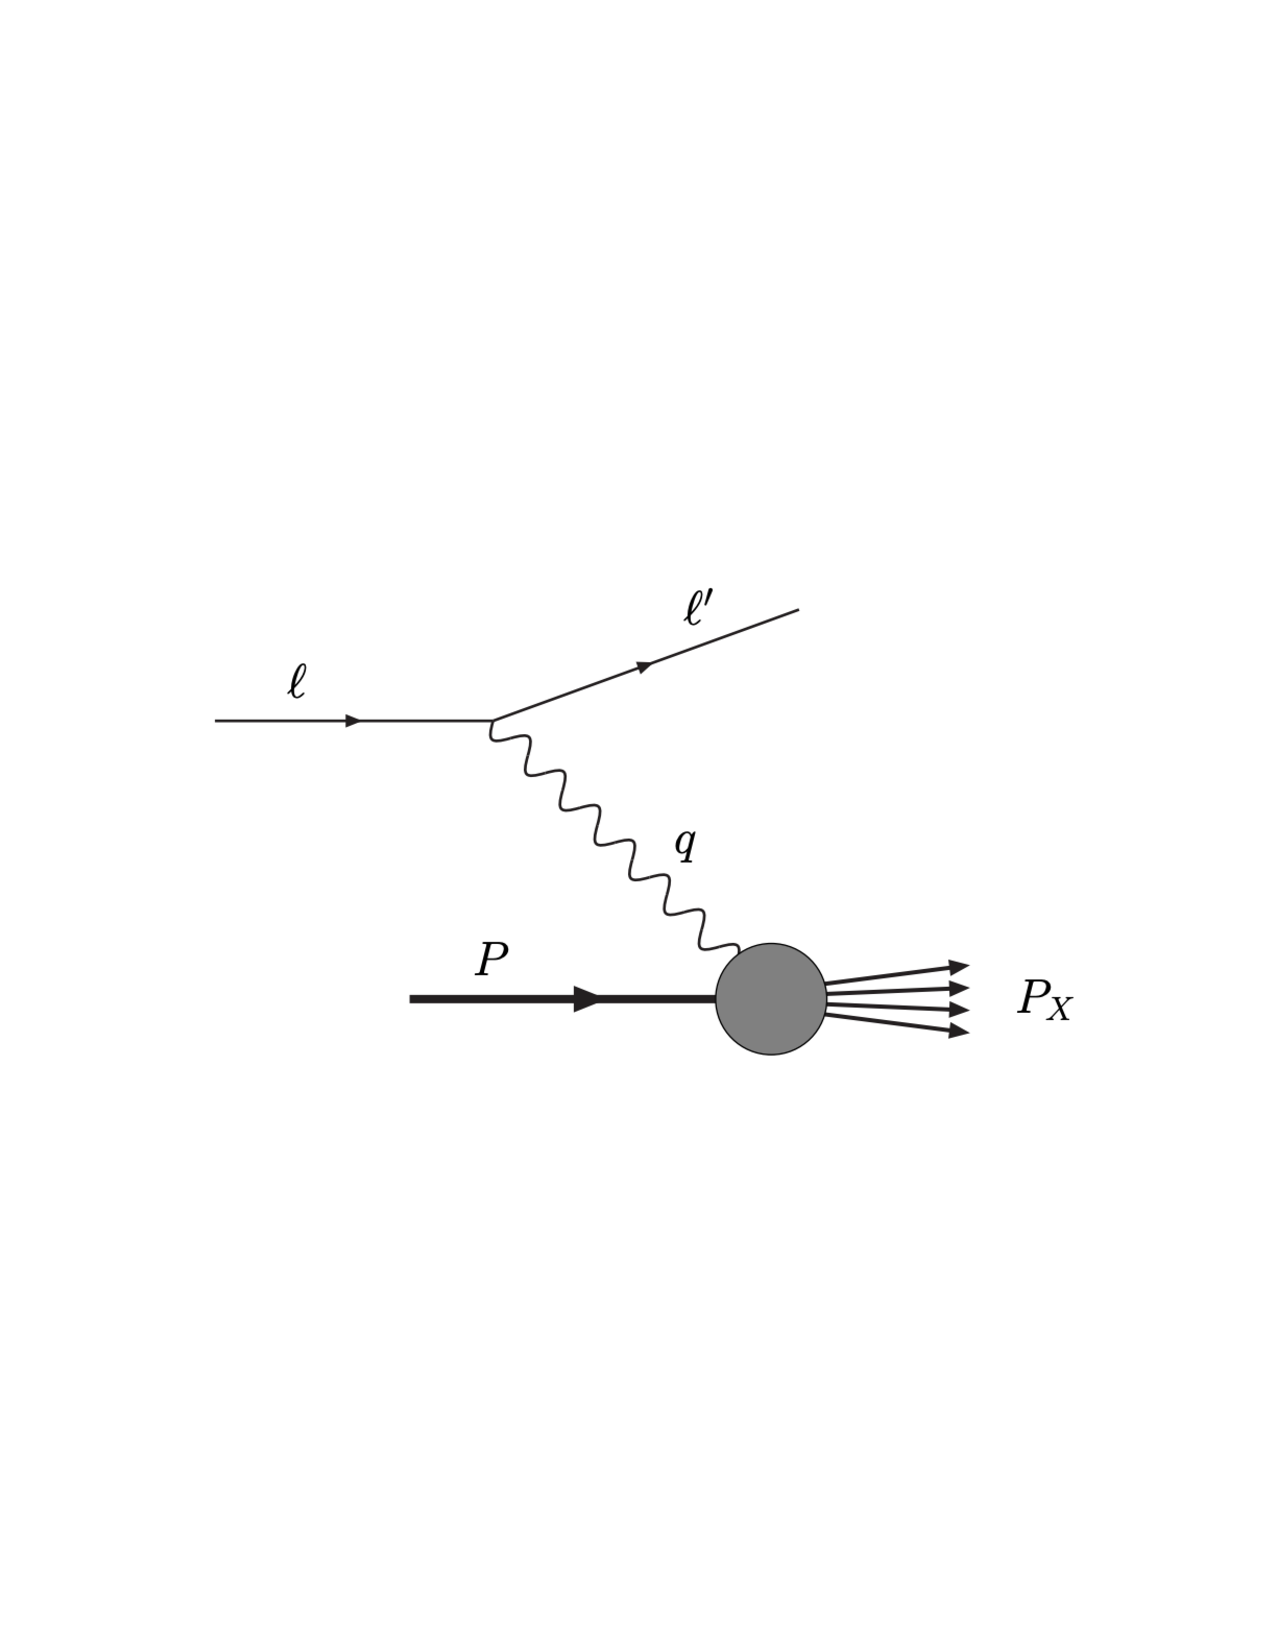
\includegraphics[width=0.5\textwidth, trim=3cm 9cm 3cm 9cm, clip]{DIS_LO}
  \caption{The leading order Feynman diagram for deep inelastic scattering}
  \label{fig::DIS_LO}
\end{figure}

DIS is traditionally studied with a high energy lepton beam and a fixed nuclear
target.  The initial state kinematics are described by

\begin{equation}
  s = (\ell+P)^2 \quad \mathrm{or} \quad E,
\end{equation}
\noindent
where $s$ is the center of mass energy and $E$ is the energy of the lepton beam.
The detected reaction kinematics in the lab frame are described by

\begin{multicols}{2}
  \noindent
  \begin{equation}
    \label{equ::DIS_Q2}
    Q^2 = -q^2 = -(\ell - \ell')^2 \approx EE'(1-\cos\theta )
  \end{equation}
  \begin{equation}
      \label{equ::BjorkenX}
      x = \frac{Q^2}{2P \cdot q} = \frac{Q^2}{2M\nu}
  \end{equation}
\end{multicols}

\begin{multicols}{2}
  \noindent
  \begin{equation}
    \nu = E - E'
  \end{equation} 
  \begin{equation}
    \label{equ::inelasticity}
    y = \frac{P \cdot q}{P \cdot \ell} = \frac{E - E'}{E} = \frac{\nu}{E}
  \end{equation} 
\end{multicols}

\begin{multicols}{2}
  \noindent
  \begin{equation}
    \label{equ::DIS_W}
    W^2 = (P+q)^2
  \end{equation}
\end{multicols}

\noindent
where $q$ is the virtual photon four momentum, $E'$ is the scattered leptons
energy, $x$ is Bjorken x, $\nu$ is the change in energy of the scattered lepton,
$y$ is the inelasticity and $W^2$ is invariant mass of hadron final state.  In
the last relation from Eq.~\ref{equ::DIS_Q2}, $\theta$ is the scattering angle
of the lepton with respect to the beam and the approximation is only true when
the lepton mass is assumed to be zero.  In Eq.~\ref{equ::BjorkenX}, $M$ is the
nucleon mass.  In the parton model, section~\ref{sec::parton_model}, $x$ has the
interpretation as being the momentum fraction of the struck parton with respect
to its parent hadron and therefore $x$ ranges between 0 and 1.  The
inelasticity, $y$, measure the proportional lepton energy reduction and
therefore takes on a value between 0 and 1.

The process is called deep if $Q^2 >> M^2$ and inelastic if $y < 1$.  For
practical purposes in experiments, the deep inelastic criteria corresponds to a
$Q^2 > 1~GeV$ and $W^2 > M^2$.  As can be seen in
Eq.~[\ref{equ::DIS_Q2}-\ref{equ::DIS_W}], not all the variables are independent.
DIS is described by two independent variables usually given by ($x$, $Q^2$) or
($x$, $y$).  For reference, in the limit as $y \to \; 1$ the process becomes
elastic scattering and can then be described by only one independent variable.

The cross-section for DIS is defined as~\cite{Barone:2001sp}
\begin{equation}
  \label{equ::DIS_xsection}
  \mathrm{d}\sigma =
  \frac{1}{4P\cdot \ell}\frac{e^4}{Q^4} L_{\mu\nu}W^{\mu\nu}
  2\pi\frac{\mathrm{d}^3\ell'}{(2\pi)^32E'}
\end{equation}
\noindent
where $L_{\mu\nu}$ is the leptonic tensor and $W^{\mu\nu}$ is the hadronic
tensor.  The leptonic tensor describes free leptons and can therefore be
calculated in perturbation theory.  It can be decomposed into a systematic
spin-independent tensor and an anti-symmetric spin-dependent tensor.  Summing
over all the possible spins of the lepton beam, the leptonic tensor is

\begin{equation}
  L_{\mu\nu} = 2\Big(\ell_{\mu}\ell'_{\nu} + \ell_{\nu}\ell'_{\mu} -
  g_{\mu\nu}\ell \cdot \ell' \Big) +
  2m\epsilon_{\mu\nu\rho\sigma}s^{\rho}q^{\sigma}
\end{equation}
\noindent
where $m$ is the lepton mass and $s^{\rho}$ is the spin four vector of the
lepton.

Generically the hadronic tensor is defined as
\begin{equation}
  W^{\mu\nu} = \frac{1}{2\pi}
  \int \mathrm{d}^4\xi e^{iq \cdot \xi}
  \langle PS | J^{\mu}(\xi)J^{\nu}(0) | PS \rangle
\end{equation}
\noindent
where $J$ is an electromagnetic current and $|PS \rangle$ represents the nucleon
with momentum $P$ and spin $S$.  The hadronic tensor describes a hadron bound
together by quantum chromo-dynamics (QCD).  As of yet there is no known
technique for calculating the hadronic tensor in a perturbation theory or
otherwise.  Instead the hadronic tensor can be written in the most general
Lorentz invariant form using structure functions to parameterize the
non-perturbative nature of the tensor.  With the use of these structure
functions, the differential DIS cross-section can be written
\begin{equation}
  \label{equ::DIS_diffxsection}
  \frac{\mathrm{d}\sigma}{\mathrm{d}x\mathrm{d}y} =
  \frac{8\pi\alpha^2ME}{Q^4}
  \Big\{
  xy^2F_1(x, Q^2) + \Big(1-y\Big)\frac{F_2(x, Q^2)}{x}
  + c_1(y, \frac{Q^2}{\nu}) g_1(x, Q^2) + c_2(y, \frac{Q^2}{\nu}) g_2(x, Q^2)
  \Big \}
\end{equation}
\noindent
where $\alpha$ is the electromagnetic coupling constant; $F_1$, $F_2$, $g_1$,
$g_2$ are structure functions; and $c_1$ and $c_2$ are functions which depend on
the polarization of the target.  The SLAC collaboration measured the structure
functions, $F_1$ and $F_2$, and found mild variations as a function
$Q^2$~\cite{Bloom:1969kc,Breidenbach:1969kd}.  This phenomenon now known as
Bjorken scaling lead to the theory of the parton model~\cite{Bjorken:1969ja}.
Fig.~\ref{fig::F2} shows the $F_2$ structure function which is approximately
constant as a function of $Q^2$.

\begin{figure}[h!t]
  \centering
  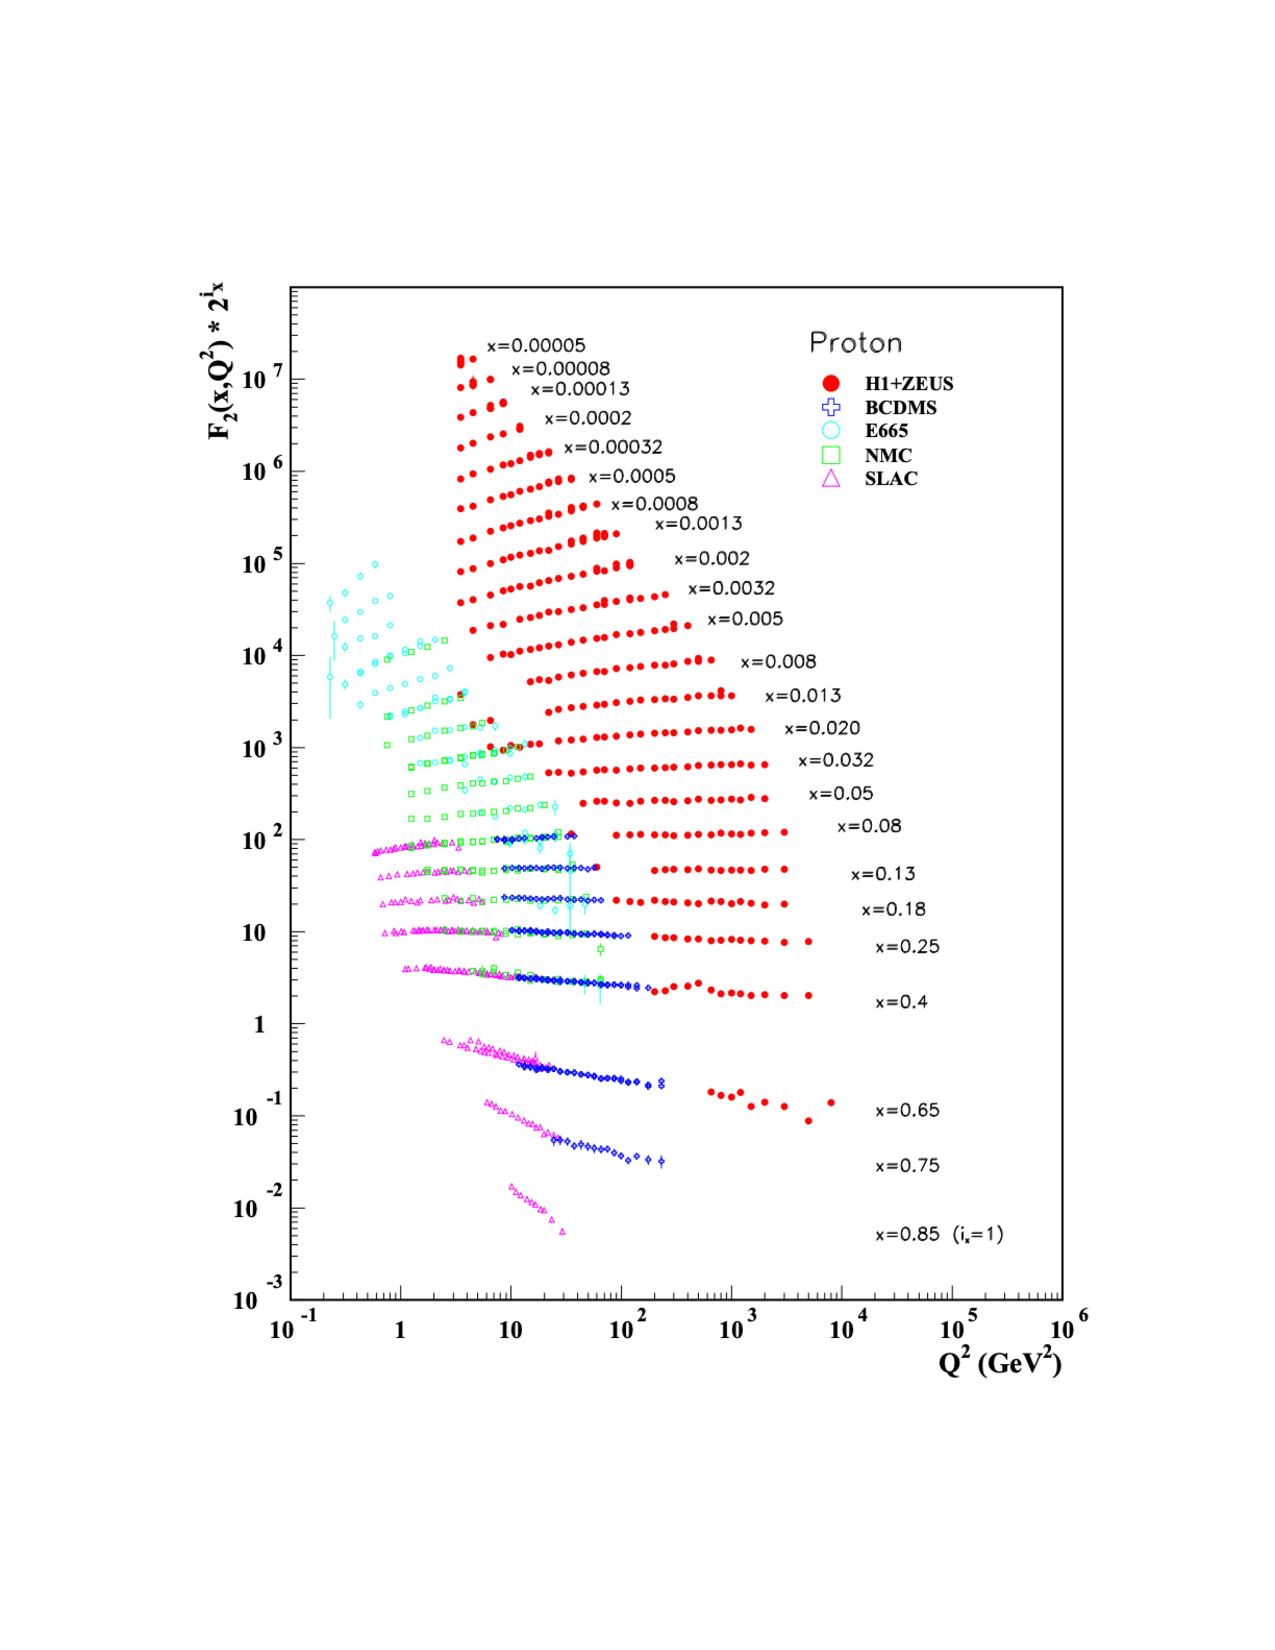
\includegraphics[width=0.5\textwidth, trim=3cm 4cm 3cm 4cm, clip]{F2}
  \caption{The $F_2$ structure function measured by several experiments.  Note
    that the data is shifted up by a factor $2^{i_x}$ to see the $x$ dependence.
    Image taken from~\cite{Tanabashi:2018oca}}
  \label{fig::F2}
\end{figure}


\section{The Parton Model} \label{sec::parton_model}
The parton model is described in what is called an infinite momentum frame where
the nucleon is moving which large momentum.  In the parton model the nucleon, in
high energy scattering processes, is considered to be composed of point like
constituent mass-less particles called partons.  At high energy scattering the
QCD strong force binding the partons becomes asymptotic small and therefore the
partons appear to be free.  The cross-section in DIS can then be described as a
lepton scattering incoherently off a free parton in the nucleon.  In the parton
model the hadron tensor for scattering off a quark can be written
as~\cite{Barone:2001sp}

\begin{dmath}
  W^{\mu\nu} = \frac{1}{2\pi} \sum_q e_q^2 \sum_X
  \int \frac{\mathrm{d}^3 P_X}{(2\pi)^32E_X}
  \int \frac{\mathrm{d}^4k}{(2\pi)^4}
  \int \frac{\mathrm{d}^4k'}{(2\pi)^4} \delta(k^{\prime2}) \times
       [\bar{u}(k')\gamma^{\mu}\langle X | u(k) | PS \rangle]*
       [\bar{u}(k')\gamma^{\nu}\langle X | u(k) | PS \rangle]
       \times (2\pi)^4\delta^4(P-k-P_X)(2\pi)^4\delta^4(k+q-k'),
\end{dmath}
\noindent
where $e_q$ is the electric charge of quark flavor $q$; and $u$ and $\bar{u}$
are free Dirac spinors.  This hadronic tensor can be simplified by introducing
the quark-quark correlation matrix as

\begin{equation}
  \Theta_{ij}(k, P, S) =
  \sum_X \int \frac{\mathrm{d}^3 P_X}{(2\pi)^32E_X}(2\pi)^4\delta^4(P-k-P_X)
  \times \langle PS | \phi_j(0) | X \rangle \langle X | \phi_i(0) | PS \rangle,
\end{equation}
\noindent
where $\phi(\xi) = e^{-ip \cdot \xi}u(p)$ is a quark field.  Using the
quark-quark correlation matrix, the hadronic tensor can be written as

\begin{equation}
  W^{\mu\nu} = \sum_q e_q^2 \int \frac{\mathrm{d}^4k}{(2\pi)^4}
  \int \frac{\mathrm{d}^4k'}{(2\pi)^4} \delta(k^{\prime2})
  (2\pi)^4\delta^4(k+q-k')\times \mathrm{Tr}
  [ \Theta \gamma^{\mu}\slashed{k'}\gamma^{\nu} ].
\end{equation}
\noindent
In the cases of unpolarized or longitudinally polarized DIS the lead order
contributing terms from the quark-quark correlator
are~\cite{Mulders:1995dh,Boer:1997nt,Bacchetta:2006tn}

\begin{equation}
  \label{equ::simpleQQcorr}
  \Theta = \frac{1}{2}
  \Big(
  f_1(x)\slashed{P} +
  g_{1L}(x)\lambda\gamma_5\slashed{P}
  \Big)
\end{equation}
\noindent
where $\lambda$ is the longitudinal polarization of the hadron.  The hadronic
tensor simplifies to a symmetric contribution and an anti-symmetric
contribution~\cite{Barone:2001sp}

\begin{equation}
  \label{equ::simpleHadronTensor}
  W^{\mathrm{symmetric}}_{\mu\nu} = \frac{1}{P\cdot q} \sum_q e_q^2
  \Big( (k_{\mu}+q_{\mu})P_{\nu} + (k_{\nu}+q_{\nu})P_{\mu}-g_{\mu\nu}
  \Big) f_1^q(x),
\end{equation}
\begin{equation}
  W^{\mathrm{anti-symmetric}}_{\mu\nu} =
  \lambda\epsilon_{\mu\nu\rho\sigma}(k_{\nu}+q_{\nu})P^{\rho}\sum_q e^2_q
  g^q_{1L}(x),
\end{equation}
\noindent
where in Eq.~\ref{equ::simpleQQcorr} $f_1$ and $g_1$ are two parton distribution
functions (PDFs).  $f_1$ is interpreted as the quark number density and $g_{1L}$
is interpreted as the total quark helicity distribution in a hadron.  $f_1$ is
then refers to the density of unpolarized quarks in a hadron and $g_{1L}$ refers
to the density of quarks longitudinally polarized in the same longitudinal
direction as the hadron.  To make this explicit, $f_1$ and $g_{1L}$ can be
written

\begin{multicols}{2}
  \noindent
  \begin{equation}
    f_1 = f_1^{+} + f_1^{-},
  \end{equation}
  \begin{equation}
    g_{1L} = f_1^{+} - f_1^{-},
  \end{equation}
\end{multicols}
\noindent
where + and - denote the helicity.  To be clear the parton distribution $g_{1L}$
is not the same as the structure function $g_1$.

The unpolarized quark number density, $f_1$, has been extracted from global
analysis of several experiments~\cite{Rojo_2015}.  Fig.~\ref{fig::NNPDF_10GeV}
shows the current $xf_1$ values and confidence intervals for different quarks
and gluons specifically in the proton.

\begin{figure}[h!t]
  \centering 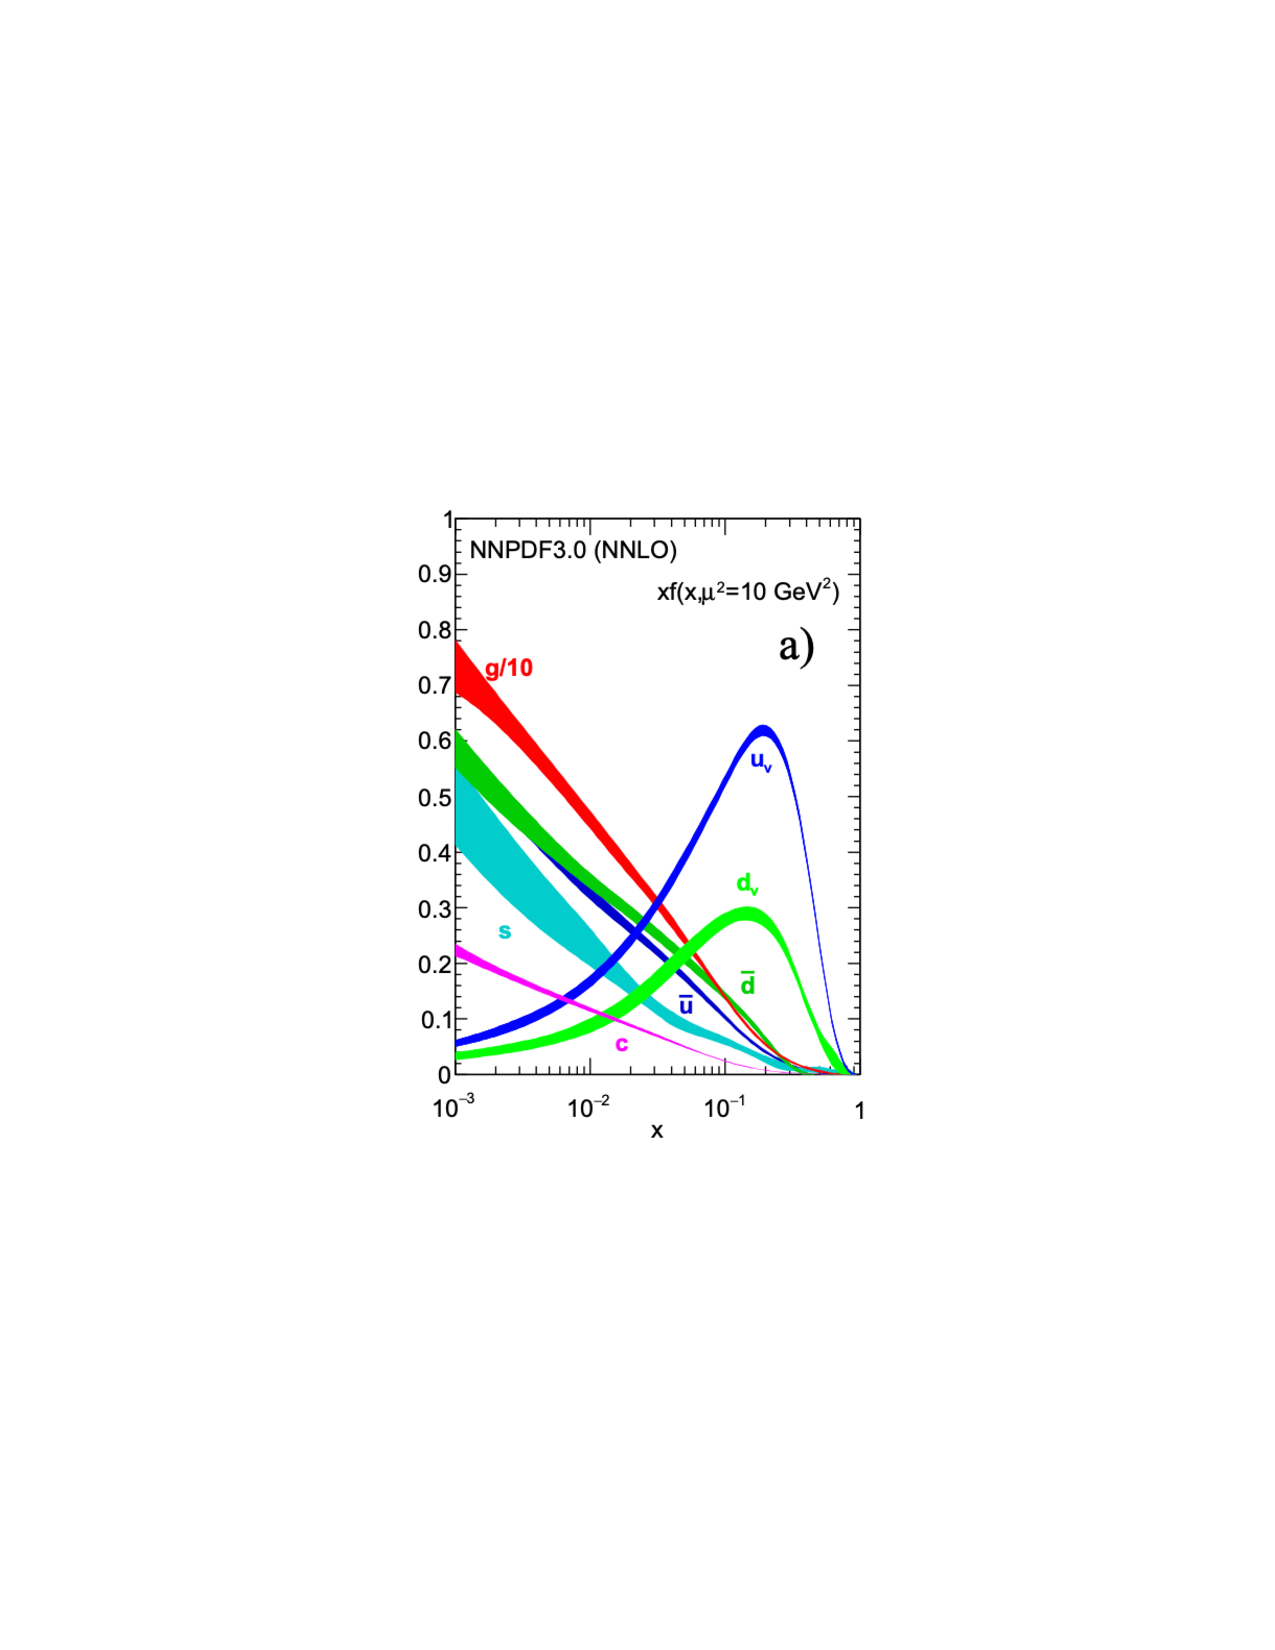
\includegraphics[width=0.5\textwidth,trim=6cm 9cm 6cm 8cm,
    clip]{NNPDF_10GeV}
  \caption{The unpolarized parton distribution functions times the momentum
    fraction.  The different color correspond to different quarks or gluons.
    Image taken from~\cite{Tanabashi:2018oca}}
  \label{fig::NNPDF_10GeV}
\end{figure}

The longitudinal spin structure, $g_{1L}$ has also been measured at SMC, HERMES,
and COMPASS~\cite{Adeva:1997is,PhysRevLett.92.012005,Savin:2011zz}.  The global
analysis fit is shown in Fig.~\ref{fig::Proton_g1L} using the parameterizations
from NNPDF2014, AAC2008, DSSV2008 and
LSS2010~\cite{Harland-Lang:2016yfn,Abt:2016vjh,Nocera:2014gqa,Hirai:2008aj}.

\begin{figure}[h!t]
  \centering 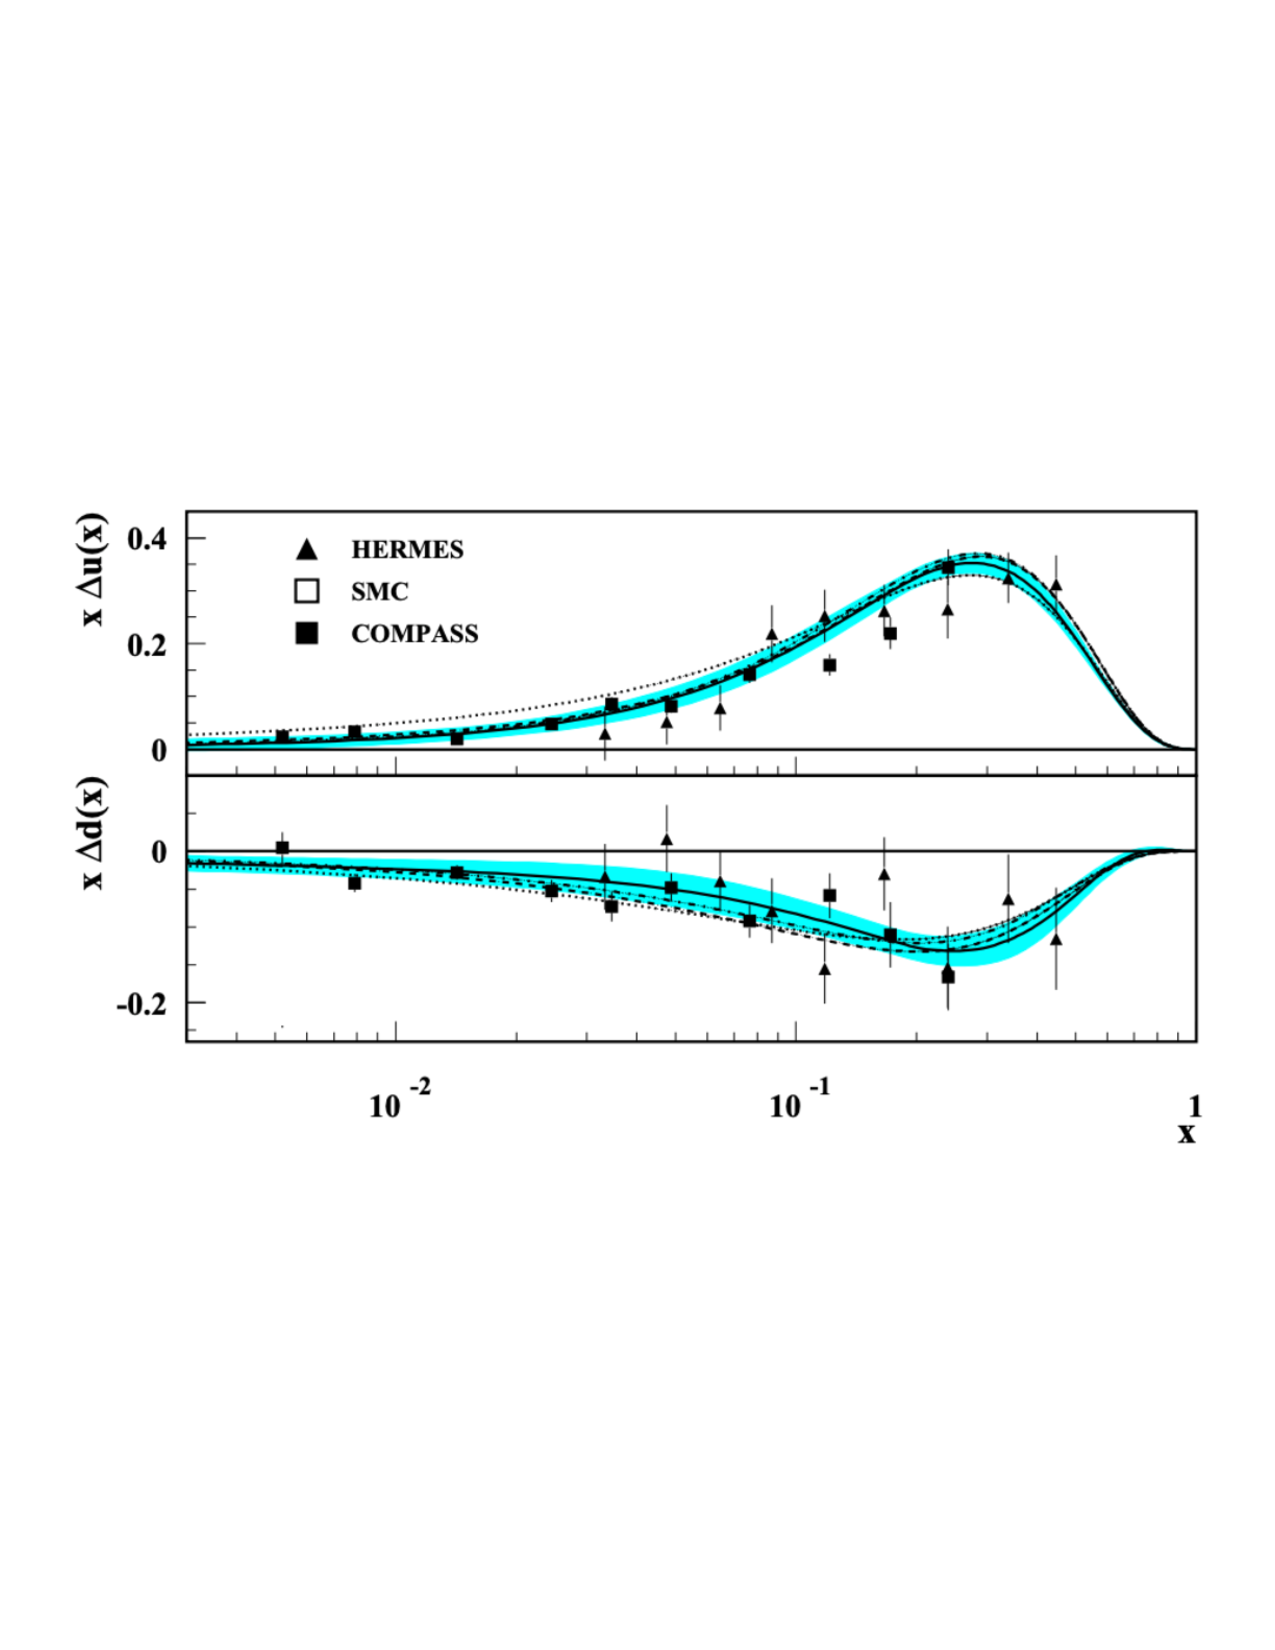
\includegraphics[width=0.5\textwidth,trim=1cm 8cm 1cm 8cm,
    clip]{Proton_g1L}
  \caption{The longitudinally polarized parton distribution functions times the
    momentum fraction for the u-quark (top) and the d-quark (bottom).  Image
    taken from~\cite{Tanabashi:2018oca}}
  \label{fig::Proton_g1L}
\end{figure}

In the parton model the structure function $F_1$ and $F_2$ are related to each
other and to the unpolarized quark number as
\begin{equation}
  F_2(x) = 2xF_1(x) = \sum_q e_q^2x\Big(f^q_1 + f^{\bar{q}}_1 \Big)
\end{equation}
which is known as the Callan-Gross relation~\cite{PhysRevLett.22.156}.  As well
the structure function $g_1$ is related to the helicity distribution, $g_{1L}$,
as
\begin{equation}
  g_1(x) = \frac{1}{2} \sum_q e^2_q g_{1L}(x).
\end{equation}


\section{Transverse Momentum Dependence}
The transverse momentum of the partons is integrated over when measuring the DIS
process.  This is because only the scattered lepton is measured and any
transverse parton motion cannot be measured.  The Drell-Yan
process~\ref{sec::DY} and the SIDIS process~\ref{sec::SIDIS} however are
sensitive to the internal transverse momentum of the partons.  In the limit of
small transverse momentum compared to the virtual photon momentum and including
the transverse parton momentum, the most generic leading order quark-quark
correlator can be written~\cite{Mulders:1995dh,Boer:1997nt,Bacchetta:2006tn}

\begin{dmath}
  \label{equ::GeneralQQcorrelator}
  \Theta = \frac{1}{2}\Big[ f_1(x,k_{\bot})\slashed{P} +
    \frac{1}{M}h_1^{\bot}(x,k_{\bot})\sigma^{\mu\nu}k_{\mu}P_{\nu} +
    g_{1L}(x,k_{\bot})\lambda\gamma_5\slashed{P} +
    \frac{1}{M}g_{1T}(x,k_{\bot})\gamma_5\slashed{P}(k_{\bot} \cdot S_{\bot}) +
    \frac{1}{M}h_{1L}(x,k_{\bot})\lambda
    i\sigma_{\mu\nu}\gamma_5P^{\mu}k_{\bot}^{\nu} +
    h_1(x,k_{\bot})i\sigma_{\mu\nu}\gamma_5P^{\mu}S_{\bot}^{\nu} +
    \frac{1}{M^2}h_{1T}^{\bot}(x,k_{\bot})i\sigma_{\mu\nu}\gamma_5P^{\mu} \Big(
    k_{\bot} \cdot S_{\bot}k_{\bot}^{\nu} - \frac{1}{2}k_{\bot}^2S_{\bot}^{\nu}
    \Big ) +
    \frac{1}{M}f_{1T}^{\bot}(x,k_{\bot})\epsilon^{\mu\nu\rho\sigma}\gamma_{\mu}P_{\nu}k_{\rho}S_{\sigma}
    \Big],
\end{dmath}
\noindent
where $k_{\bot}$ denotes the transverse parton momentum and $S_{\bot}$ denotes
the transverse hadron spin.  Eq.~\ref{equ::GeneralQQcorrelator} includes eight
transverse momentum dependent (TMD) PDFs which are functions of $x$ and
$k_{\bot}$.  The notation used to depict the TMDs functions is the so-called
Amsterdam notation.  The letters represent the different quark polarizations
where $f, g, h$ stand for unpolarized, longitudinally polarized and transversely
polarized respectively.  The subscript 1 denotes leading order and the
subscripts $T$ and $L$ denote a transversely polarized hadron and a
longitudinally polarized hadron respectively.  Finally the superscript $\bot$
denotes that the distribution is an odd function of $k_{\bot}$ and therefore is
zero when integrated over the parton transverse momentum.  Fig.~\ref{fig::TMDs}
organizes the TMDs by nucleon and quark polarizations and gives a visual of each
TMD's interpretation.

\begin{figure}[h!t]
  \centering
  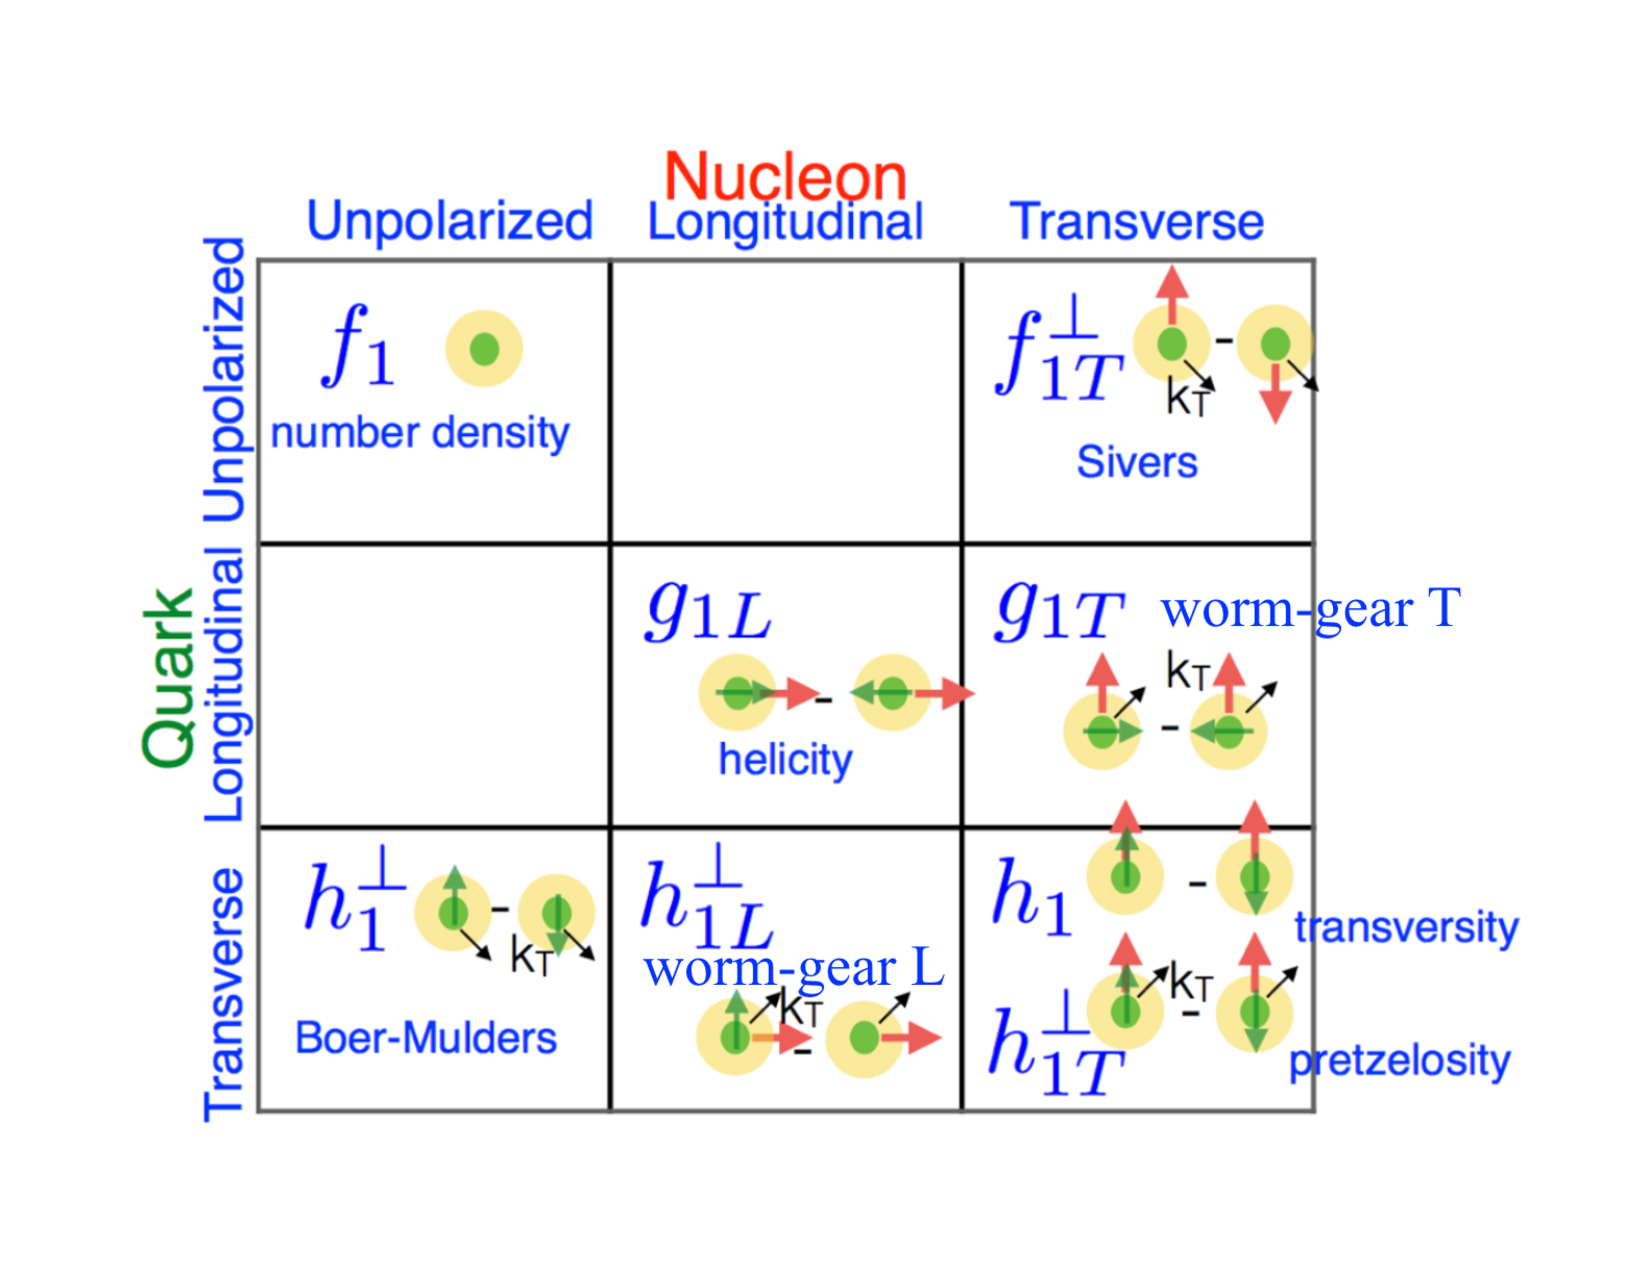
\includegraphics[width=0.6\textwidth, trim=2cm 2cm 2cm 2cm,clip]{TMDs}
  \caption{The eight TMDs needed to describe a spin 1/2 nucleon at leading
    order.  The columns represent the different nucleon polarization and the
    rows represent the different quark polarizations.  The individual figures
    give a visual of the TMD's interpretation.}
  \label{fig::TMDs}
\end{figure}

\subsection{Sivers Distribution}
The Sivers TMD was first purposed to explain large nucleon spin-dependent
asymmetries~\cite{Sivers}.  The interpretation of the Sivers TMD, {\siv}, is
that it gives a correlation between transverse spin of the parent hadron and
transverse momentum of parton.  When viewing the hadron in the direction of it's
momentum, if {\siv} is positive then it is expected that there are more partons
with momentum going left than going right.  Intuitively a non-zero {\siv} would
then imply that the bound quarks carry orbital angular momentum.  As of yet
however, there is no theoretical link between orbital angular momentum and the
Sivers function.

The Sivers function is changes sign from naive time reversal.  Naive time
reversal is defined as reversing time but not swapping initial and final
states~\cite{Bacchetta:2006tn}.  The Sivers function is therefore said to be a
T-odd function, and as a result it was originally believe to be a forbidden
correlation.  However it was shown that the Sivers function could be non-zero
from gluon exchange during the initial state in the Drell-Yan process and during
the final state in SIDIS~\cite{Brodsky:2002cx,Brodsky:2002rv}.  Surprising it
was shown that a non-zeron Sivers function is expected to have opposite sign in
SIDIS and Drell-Yan~\cite{collins_2002}.  That is

\begin{equation}
  f_{1T}^{\bot} |_{Drell-Yan} = - f_{1T}^{\bot} |_{SIDIS}.
\end{equation}


Include information on Bohr-Mulders, transversity and prezelosity (all TSAs
determined in DY).  Give Star Sivers result.

\section{Semi-Inclusive Deep Inelastic Scattering} \label{sec::SIDIS}
Semi-Inclusive Deep Inelastic Scattering (SIDIS) is the process where a lepton
scatters electromagnetically off a nucleon and subsequently the scattered lepton
and at least one scattered hadron are detected.  As the name implies, SIDIS is
related to the DIS reaction only SIDIS includes the addition of a detected
hadron.  SIDIS is denoted as

\begin{equation}
  l(\ell, \lambda_l) + N(P, S) \rightarrow l(\ell') + h(P_h) + X(P_X),
\end{equation}
\noindent
where $\lambda_l$ is the helicity of the incoming lepton, $S$ is the spin of the
nucleon, $h$ is the detected hadron and $P_h$ is the detected hadron's four
momentum.  The leading order one photon exchange Feynman diagram for the SIDIS
process is shown in Fig.~\ref{fig::SIDIS_LO}.

\begin{figure}[h!t]
  \centering
  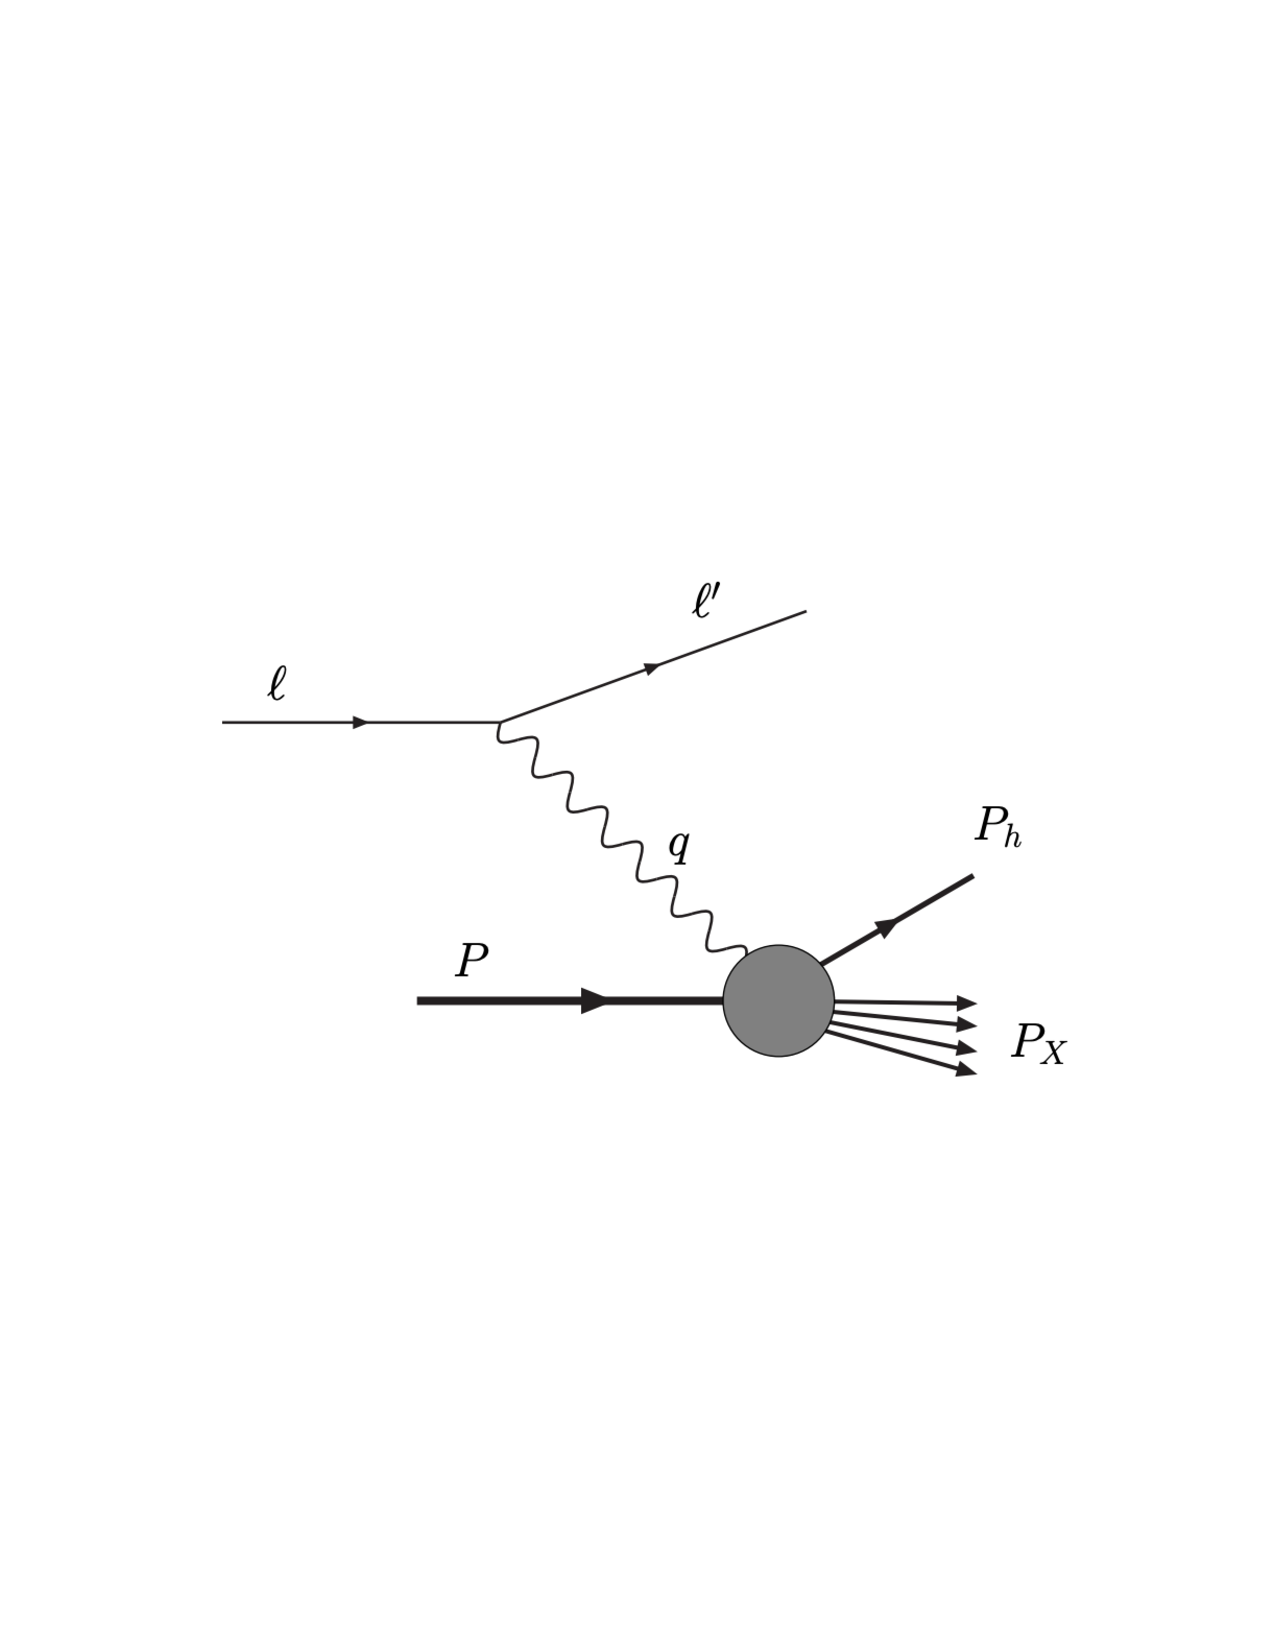
\includegraphics[width=0.5\textwidth, trim=3cm 9cm 3cm 9cm, clip]{SIDIS_LO}
  \caption{The semi-inclusive deep inelastic scattering leading order Feynman
    diagram}
  \label{fig::SIDIS_LO}
\end{figure}

In addition to the kinematic variables used to describe DIS,
Eq.~[\ref{equ::DIS_Q2}-\ref{equ::DIS_W}], one more variable is needed to
describe the SIDIS process,
\begin{equation}
  z = \frac{P \cdot P_h}{P \cdot q} \quad \substack{lab \\frame\\ =} \quad
  \frac{E_h}{E-E'},
\end{equation}
\noindent
which is interpreted as the fraction of possible energy the detected hadron
can obtain.  The transverse spin-dependent SIDIS cross-section can be described
in a model independent way using structure functions as~\cite{Bacchetta:2006tn}

\begin{align}
  \frac{d\sigma}{dx \, dy\, d\psi \,dz\, d\phi_h\, d P_{h\perp}^2} &=
  \frac{\alpha^2}{x y Q^2}\,
  \frac{y^2}{2\,(1-\varepsilon)}\,  \biggl( 1+\frac{\gamma^2}{2x} \biggr)\,
  \Biggl\{
  F_{UU ,T}
  + 
  \varepsilon
  F_{UU ,L}
  + \sqrt{2\,\varepsilon (1+\varepsilon)}\,\cos\phi_h\,
  F_{UU}^{\cos\phi_h}
  \nonumber \\  & 
  + \varepsilon \cos(2\phi_h)\, 
  F_{UU}^{\cos 2\phi_h}
  + \lambda_l\, \sqrt{2\,\varepsilon (1-\varepsilon)}\, 
  \sin\phi_h\, 
  F_{LU}^{\sin\phi_h}
  \phantom{\Bigg[ \Bigg] }
  \nonumber \\  & 
  + |S_\perp|\, \Bigg[
    \sin(\phi_h-\phi_S)\,
    \Bigl(F_{UT ,T}^{\sin\left(\phi_h -\phi_S\right)}
    + \varepsilon\, F_{UT ,L}^{\sin\left(\phi_h -\phi_S\right)}\Bigr)
    \nonumber \\  & \quad  \qquad \qquad
    + \varepsilon\, \sin(\phi_h+\phi_S)\, 
    F_{UT}^{\sin\left(\phi_h +\phi_S\right)}
    + \varepsilon\, \sin(3\phi_h-\phi_S)\,
    F_{UT}^{\sin\left(3\phi_h -\phi_S\right)}
    \phantom{\Bigg[ \Bigg] }
    \nonumber \\  & \quad \qquad \qquad
    + \sqrt{2\,\varepsilon (1+\varepsilon)}\, 
    \sin\phi_S\, 
    F_{UT}^{\sin \phi_S }
    + \sqrt{2\,\varepsilon (1+\varepsilon)}\, 
    \sin(2\phi_h-\phi_S)\,  
    F_{UT}^{\sin\left(2\phi_h -\phi_S\right)}
    \Bigg]
  \nonumber \\  &
  + |S_\perp| \lambda_l\, \Bigg[
    \sqrt{1-\varepsilon^2}\, \cos(\phi_h-\phi_S)\, 
    F_{LT}^{\cos(\phi_h -\phi_S)}
    +\sqrt{2\,\varepsilon (1-\varepsilon)}\, 
    \cos\phi_S\, 
    F_{LT}^{\cos \phi_S}
    \nonumber \\  & \quad \qquad \qquad
    +\sqrt{2\,\varepsilon (1-\varepsilon)}\, 
    \cos(2\phi_h-\phi_S)\,  
    F_{LT}^{\cos(2\phi_h - \phi_S)}
    \Bigg] \Biggr\},
  \label{equ::SIDISxsect}
\end{align}
\noindent
where
\begin{equation}
  \varepsilon =
  \frac{1-y-\frac{1}{4}\gamma^2y^2}{1-y+\frac{1}{2}y^2+\frac{1}{4}\gamma^2y^2},
\end{equation}
\noindent
and $\gamma = \frac{2Mx}{Q}$ and $\psi$ is the azimuthal scattering angle of the
lepton around the lepton beam with respect to the transverse spin direction of
the target.  The SIDIS cross-section, Eq.~\ref{equ::SIDISxsect}, is defined in
the $\gamma$-nucleon reference frame which is a target frame where the virtual
photon is along the z-axis and the xz-plane is determined by the lepton plane.
Fig.~\ref{fig::gammaNucleonFrame} shows the $\gamma$-nucleon lab frame and the
relevant azimuthal angles.

The 14 structure functions in Eq.~\ref{equ::SIDISxsect} are coefficients to the
azimuthal angles.  The structure functions are label as $F$ where the
superscript denotes which azimuthal angle coefficient they correspond to and the
three subscripts represent the beam, target and virtual photon polarization from
left to right respectively.  The subscript polarizations are $U$ for
unpolarized, $L$ for longitudinally polarized and $T$ for transversely
polarized.  The cross-section, Eq.~\ref{equ::SIDISxsect}, is determined
similarly to the DIS cross-section,Eq.~\ref{equ::DIS_diffxsection}, in that
structure functions are used to generically parameterize the hadronic tensor.

\begin{figure}[h!t]
  \centering 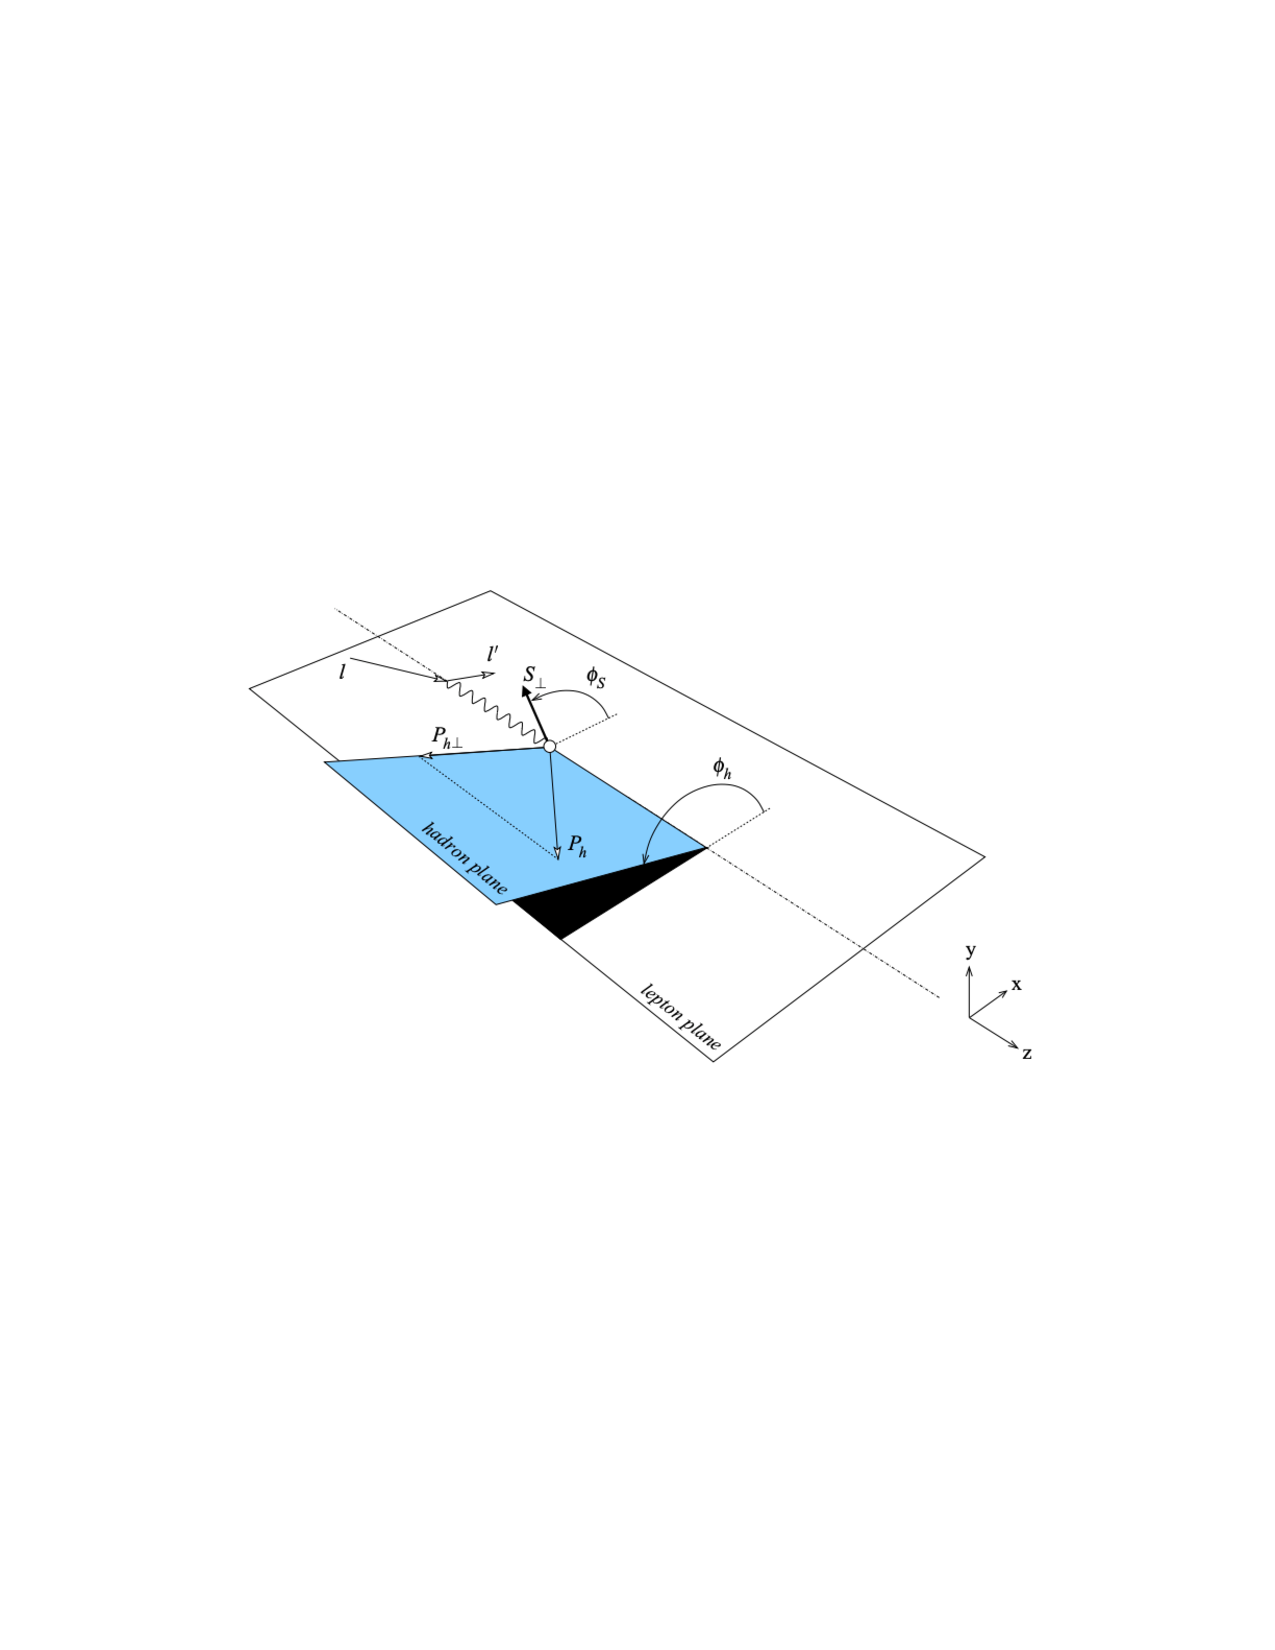
\includegraphics[width=0.6\textwidth,trim=3cm 9cm 3cm 8cm,
    clip]{gammaNucleonFrame}
  \caption{The $\gamma$-nucleon lab frame where the target nucleon is at rest
    and the virtual photon is along the z-axis.  The lepton scattering plane
    defines the xz-plane where the outgoing lepton defines the positive
    x-direction.  This image was taken from~\cite{Bacchetta:2006tn}.}
  \label{fig::gammaNucleonFrame}
\end{figure}

In the TMD regime the structure functions are related to TMD function and
fragmentation functions (FF).  That is to say where the detected hadron's
transverse momentum is small compared to the virtual photon momentum, $P_{hT} <<
Q$, the model independent structure functions are related to TMD functions.  The
structure functions are equal to a convolution of a TMD and a FF in this regime
where the convolution is defined as

\begin{equation}
  \label{equ::SIDIS_conv}
{\cal C}\bigl[ w(p_T,k_T) f D \bigr] = x \sum_q e_q^2 \int d^2 p_T d^2 k_T
\delta^{(2)}\bigl(p_T - k_T - P_{h \perp}/z \bigr) w(p_T,k_T)
f^q(x,p_T^2)D^q(z,k_T^2),
\end{equation}
\noindent
where $w$ is a weight $f$ is a TMD function and $D$ is a FF.  The relation
between structure functions and TMDs at leading order for the structure
functions related to transverse target polarization are~\cite{Bacchetta:2006tn}

\begin{align}
  \label{equ::F_UUTsinphihphis}
  F_{UT ,T}^{\sin\left(\phi_h -\phi_S\right)} &=
  {\cal C}\biggl[-\frac{\hat{h} \cdot p_T}{M} f_{1T}^{\perp } D_1\biggr]
  &\propto f_{1T}^{\perp } \otimes D_1, \\
  F_{UT ,L}^{\sin\left(\phi_h -\phi_S\right)} &= 0,\\
  F_{UT}^{\sin(\phi_h +\phi_S)} &=
  {\cal C}\biggl[-\frac{\hat{h}\cdot k_T^{}}{M_h} h_{1} H_1^{\perp }\biggr]
  &\propto h_{1} \otimes H_1^{\perp },\\
  F_{UT}^{\sin(3\phi_h -\phi_S)} &=
  {\cal C}\biggl[ \frac{2 \bigl(\hat{h}\cdot
      p_T \bigr) \bigl( \bm{p}_T\cdot k_T^{} \bigr) +\bm{p}_T^2
      \bigl(\hat{h}\cdot k_T^{} \bigr) -4 (\hat{h}\cdot p_T)^2 (\hat{h}\cdot
      k_T^{})}{2 M^2 M_h} h_{1T}^{\perp } H_1^{\perp }\biggr]
  &\propto h_{1T}^{\perp } \otimes H_1^{\perp },\\
  \label{equ::F_LTcosphihphis}
  F_{LT}^{\cos(\phi_h -\phi_S)}
  &={\cal C}\biggl[ \frac{\hat{h} \cdot p_T}{M} g_{1T}
    D_1 \biggr]
  &\propto g_{1T} \otimes D_1, 
\end{align}

\noindent
and the leading order structure functions related to an unpolarized target are

\begin{align}
  F_{UU ,T} &= {\cal C}\bigl[ f_1 D_1 \bigr] &\propto f_1 \otimes D_1, \\
  \label{equ::F_UUL}
  F_{UU ,L} &= 0,
\end{align}

\noindent
where the unit vector $\hat{h}=P_{h \perp}/|P_{h\perp}|$ and $D_1$ and
$H_1^{\perp}$ are fragmentation functions.  The fragmentation functions are
functions of $z$ and describe the probability for a quark to hadronize to a
specific hadron.  These fragmentation functions depend on the quark spin, the
hadron type and polarization and the quark $k_T$.  In
Eq.~[\ref{equ::F_UUTsinphihphis}-~\ref{equ::F_UUL}] the fragmentation
function $D_1$ refers to an unpolarized quark fragmenting to an unpolarized
hadron and $H_1^{\perp}$ refers to a transversely polarized quark fragmenting to
an unpolarized hadron.

The SIDIS cross-section, Eq.~\ref{equ::SIDISxsect}, can be rewritten in terms of
asymmetries.  These asymmetries are defined as

\begin{equation}
  A^{w_i(\phi_h, \phi_S)}_{BeamTarget} = \frac{F^{w_i(\phi_h,
      \phi_S)}_{BeamTarget}}{F_{UU,T}+\varepsilon F_{UU,L}},
  \label{equ::asymAmpSIDIS}
\end{equation}
\noindent
where $w_i(\phi_h, \phi_S)$ is the azimuthal angle associated with this
asymmetry and $Beam$ and $Target$ represent the polarization of the beam and
target.  The asymmetry amplitude, Eq.~\ref{equ::asymAmpSIDIS}, is a structure
function divide by the unpolarized structure functions.  This asymmetry
amplitude definition is defined because it is easier to measure experimentally.
In order to determine an asymmetry amplitude, the number of counts
experimentally measures can be fit using a function in the form of
Eq.~\ref{equ::SIDISxsect} with the coefficients to each azimuthal amplitude as
parameters to the fit.  The result of the fit can determine the spin-dependent
asymmetry amplitudes without needing to determine the luminosity.

COMPASS and HERMES measurements the asymmetry $A_{UT ,T}^{\sin\left(\phi_h
  -\phi_S\right)}$ from the SIDIS reaction from a proton
target~\cite{Alekseev:2008aa,Airapetian:2009ae}.  The comparison of the result
between these two collaboration is shown in Fig.~\ref{fig::SiversFromSIDIS}.
The asymmetry amplitude $A_{UT ,T}^{\sin\left(\phi_h-\phi_S\right)}$ is related
to the Sivers function and was measured to be non-zero at the level of 5\%.

\begin{figure}[h!t]
  \centering 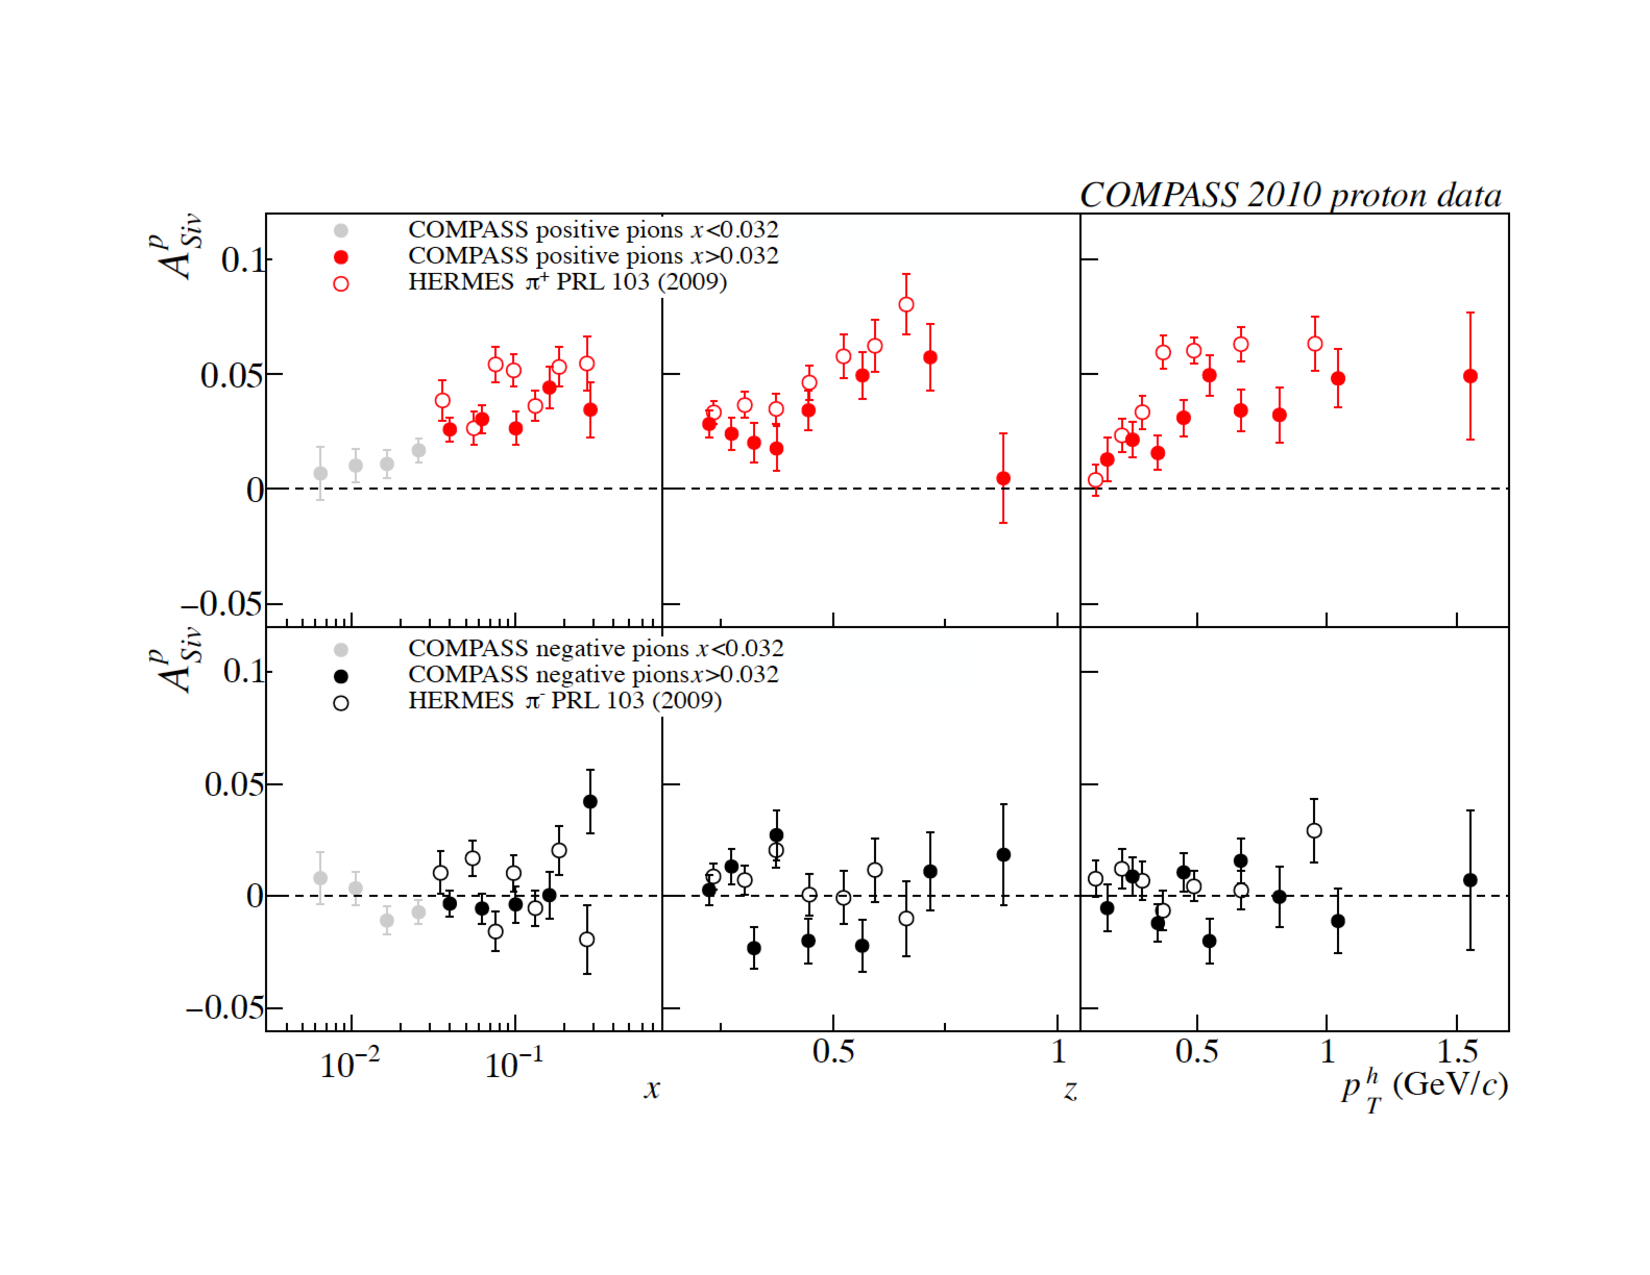
\includegraphics[width=0.6\textwidth, trim=2cm 2cm 2cm
    3cm,clip]{SiversFromSIDIS}
  \caption{The asymmetry amplitude related to the Sivers function measure by
    COMPASS~\cite{Alekseev:2008aa} and HERMES~\cite{Airapetian:2009ae}}
  \label{fig::SiversFromSIDIS}
\end{figure}

The top plots in Fig.~\ref{fig::SiversFromSIDIS} is the asymmetry for a positive
detected hadron which is dominated by u-quark scattering and therefore by the
u-quark Sivers function.  This is the case for three reasons.  Firstly because
the SIDIS reaction is weighted by charge squared which therefore makes the
u-quark scattering four times more likely.  Secondly the so-called favor FF,
where the detected hadron is the same charge as the which quark fragmented, is
larger than the unfavored FF.  Therefore a positively detected hadron most
likely resulted from a positively fragmenting quark.  Thirdly the proton target
is composed twice as many u-quarks as d-quarks in this scattering kinematic
region.  For these three reasons the results in Fig.~\ref{fig::SiversFromSIDIS}
imply that the u-quark Sivers function from the SIDIS reaction is positive.

The bottom plots in Fig.~\ref{fig::SiversFromSIDIS} suggest that the d-quark
Sivers function in the SIDIS reaction is negative.  The bottom results in
Fig.~\ref{fig::SiversFromSIDIS} are from the combination of u-quark scattering
then fragmenting unfavoredly and d-quark scattering and fragmenting favoredly.
As was mentioned the charge weighting in the SIDIS reaction and the proton quark
composition results in the u-quark scattering with a higher probability.  On the
other hand the favor FF for d-quark fragmenting to a negatively charged hadron
versus the unfavored FF for u-quark fragmenting to a negatively charged hadron
cancel the previous effect out.  Therefore results in the bottom of
Fig.~\ref{fig::SiversFromSIDIS} are for an equal combination from u-quark
scattering and d-quark scattering.  As the u-quark asymmetry amplitude is
positive, the d-quark asymmetry amplitude must therefore be negative and so also
must the d-quark Sivers function.


\section{Drell-Yan} \label{sec::DY}
The Drell-Yan process is the reaction where a quark and an anti-quark annihilate
and the end product results in two leptons.  The Drell-Yan process is denoted as

\begin{equation}
  H_a(P_a) + H_b(P_b, S) \rightarrow \gamma^* + X \rightarrow l(\ell) +
  l'(\ell') + X
\end{equation}
\noindent
where $H_a$ and $H_b$ are hadrons which carry the quark and anti-quarks and only
the target hadron, $H_b$ is considered to polarized with spin $S$.  In this
thesis the quark anti-quark pair annihilate to form a virtual photon, $\gamma^*$
and in addition the final state leptons detected are a muon and an anti-muon.
The leading order one photon exchange diagram is shown in Fig.~\ref{fig::DY_LO}.

\begin{figure}[h!t]
  \centering
  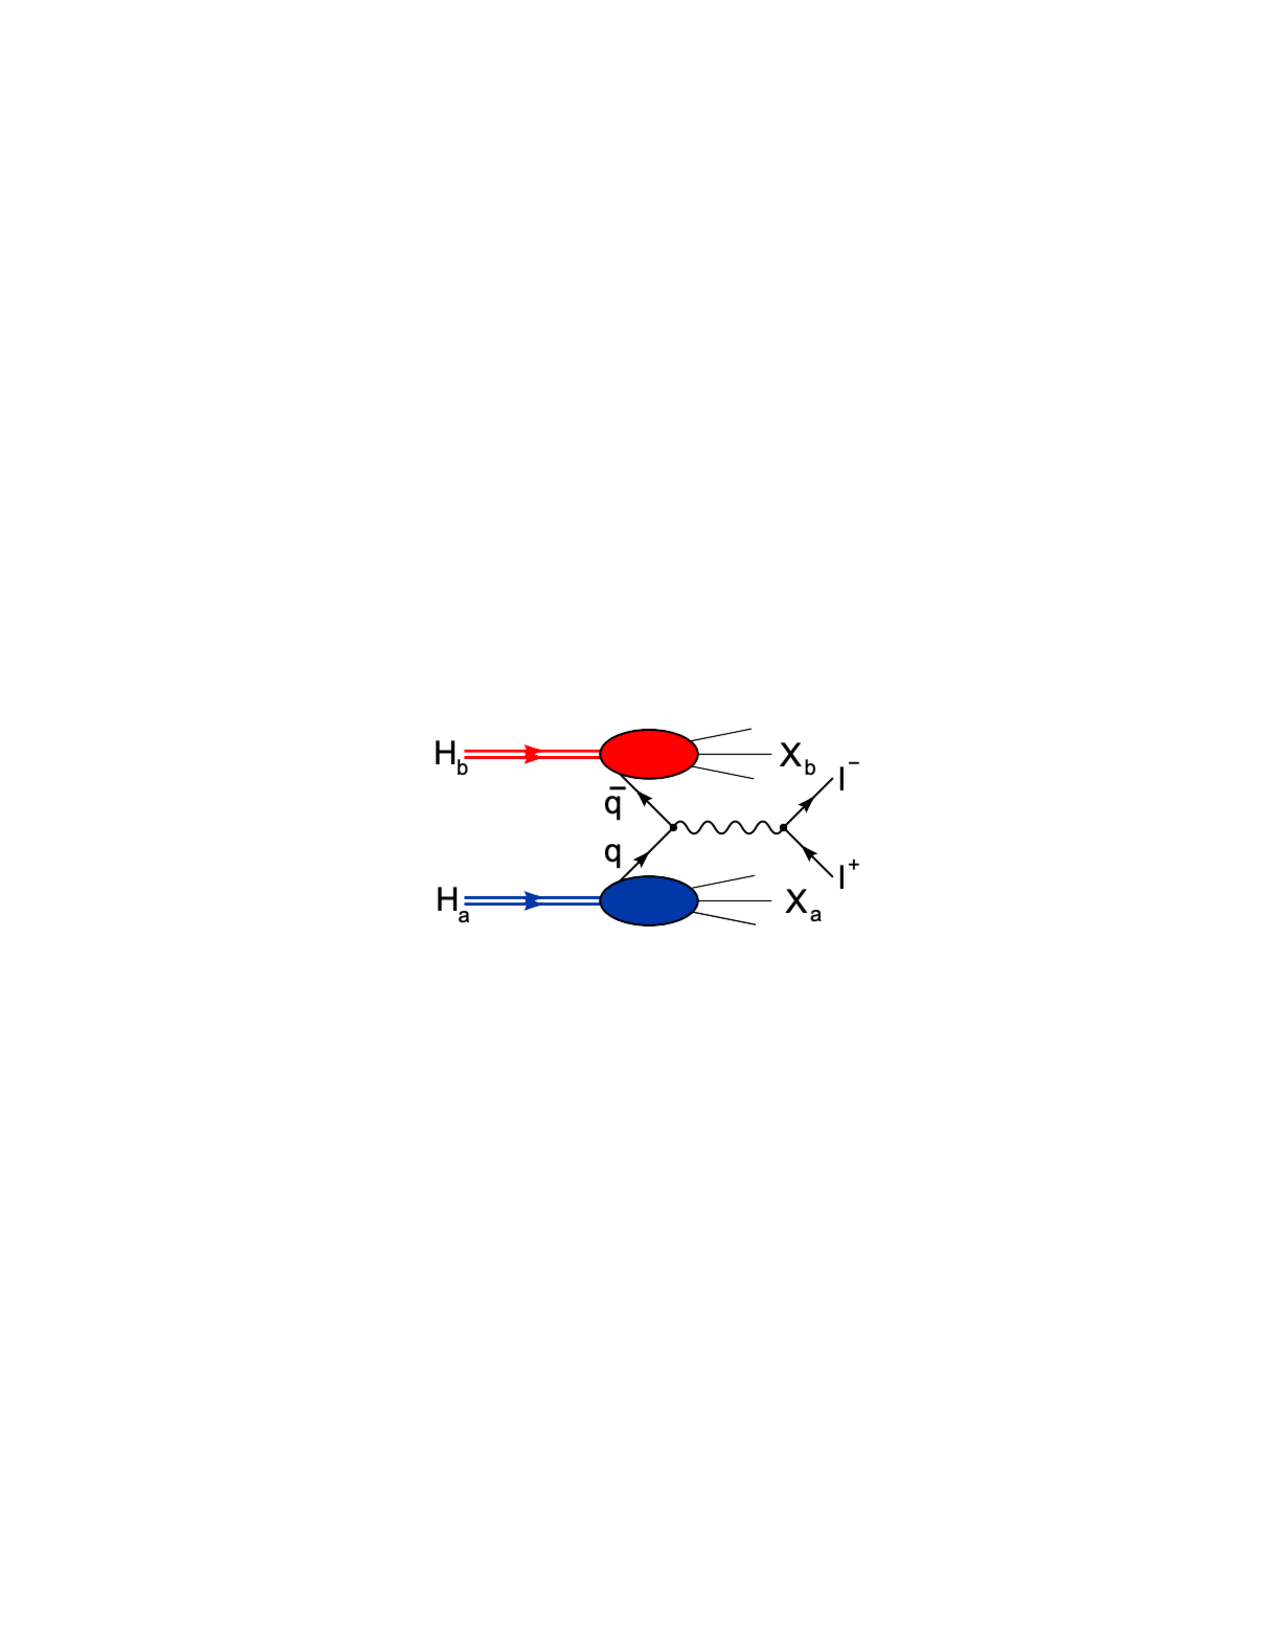
\includegraphics[width=0.45\textwidth, trim=7cm 12cm 7cm 12cm, clip]{DY_LO}
  \caption{The Drell-Yan leading order diagram}
  \label{fig::DY_LO}
\end{figure}

The angles used to define the general Drell-Yan cross-section are defined with
the use of two reference frames.  The target frame (TF),
Fig.~\ref{fig::DY_TargetFrame}, defines the $\phi_S$ angle and the Collins-Soper
(CS), Fig.~\ref{fig::DY_CSFrame}, frame defines the additional $\phi$ and
$\theta$ angles.  The $\phi_S$ angle is defined in TF as the angle between the
transverse momentum of the virtual photon and the transverse spin of the target.
The $\phi$ and $\theta$ angles, in the CS frame, are defined as the azimuthal
and polar angle of the negatively charged muon.

\begin{figure}[h!t]
  \centering
  \begin{subfigure}{.46\textwidth}
    \centering
    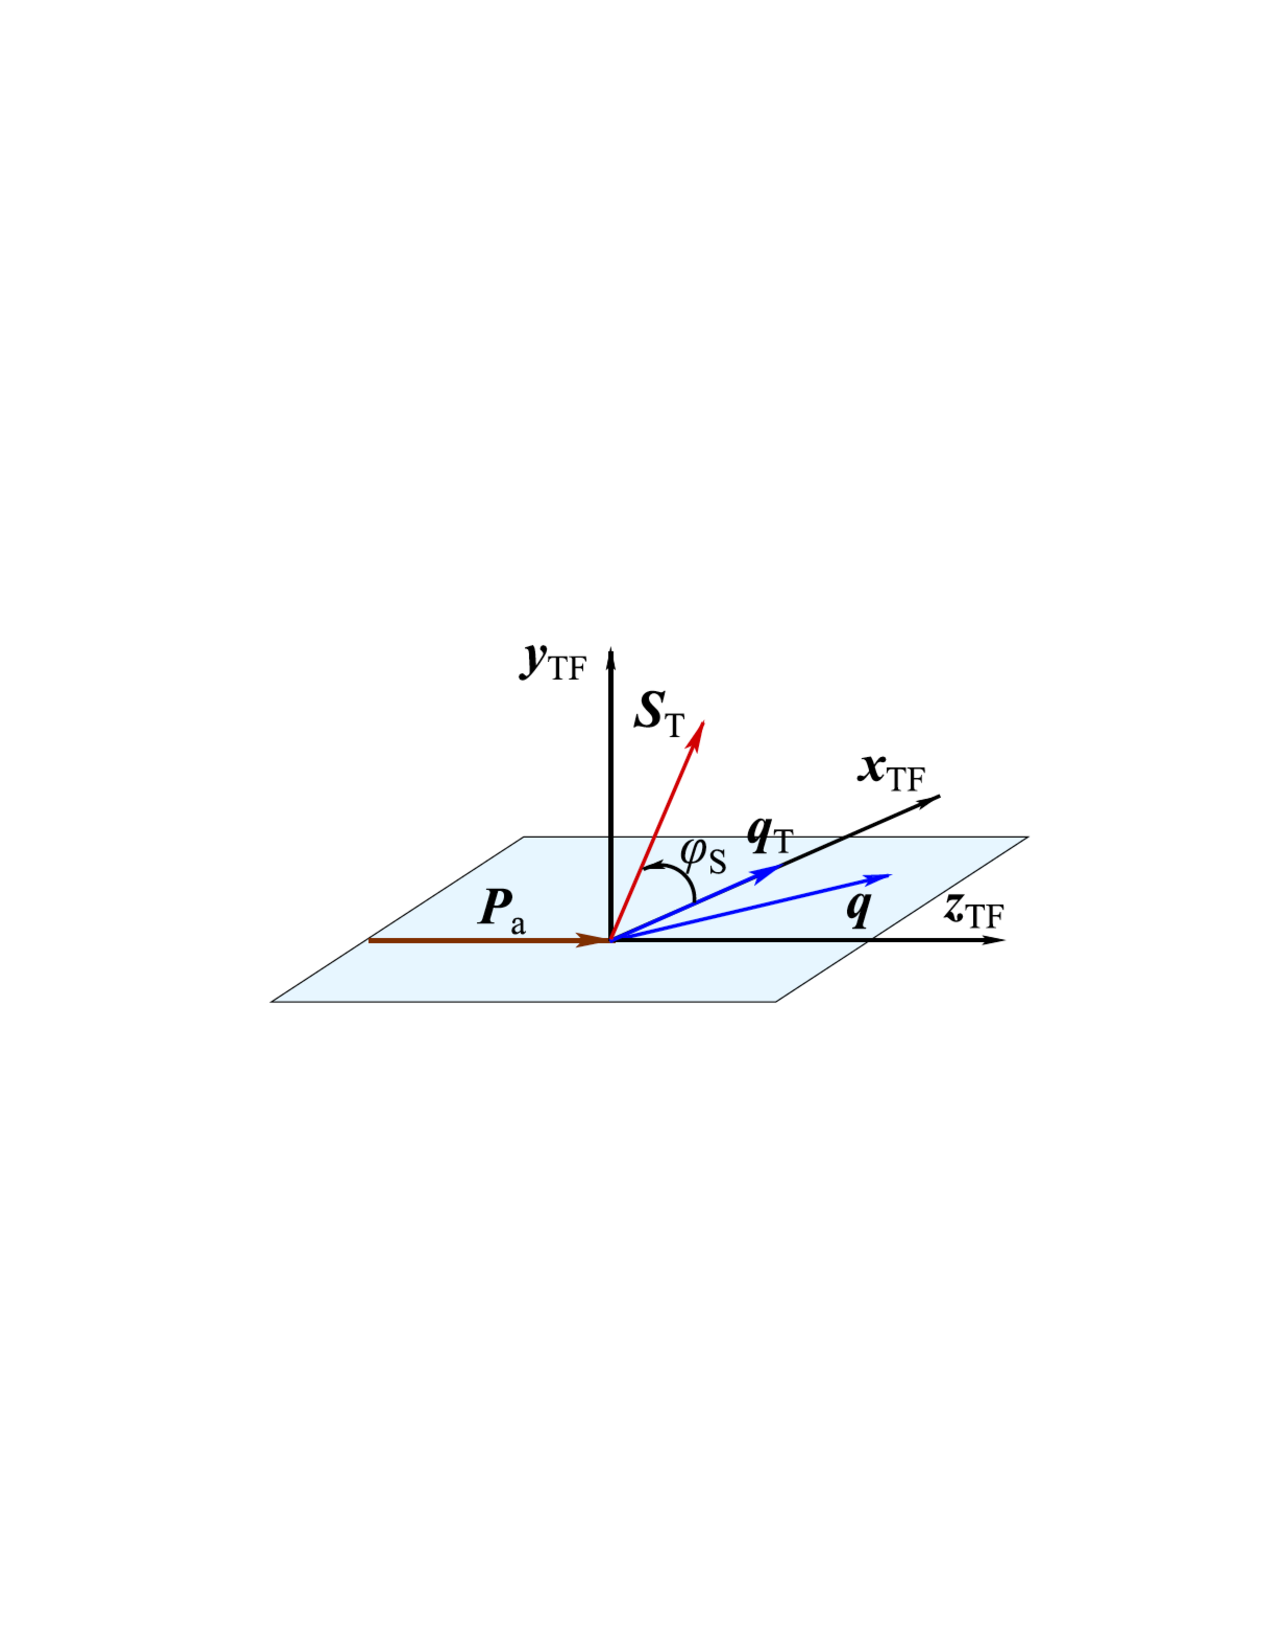
\includegraphics[width=\linewidth, trim=3cm 9cm 3cm 8cm,
      clip]{DY_TargetFrame}
    \caption{The target frame where the z-axis is along the beam and the x-axis
      is in the direction of the transverse momentum of the virtual photon.}
    \label{fig::DY_TargetFrame}%
  \end{subfigure}
  \begin{subfigure}{.02\textwidth}
    \centering
    
\includegraphics[width=\linewidth]{tmp}
    \label{fig::tmp1}%
  \end{subfigure}
  \begin{subfigure}{.46\textwidth}
    \centering
    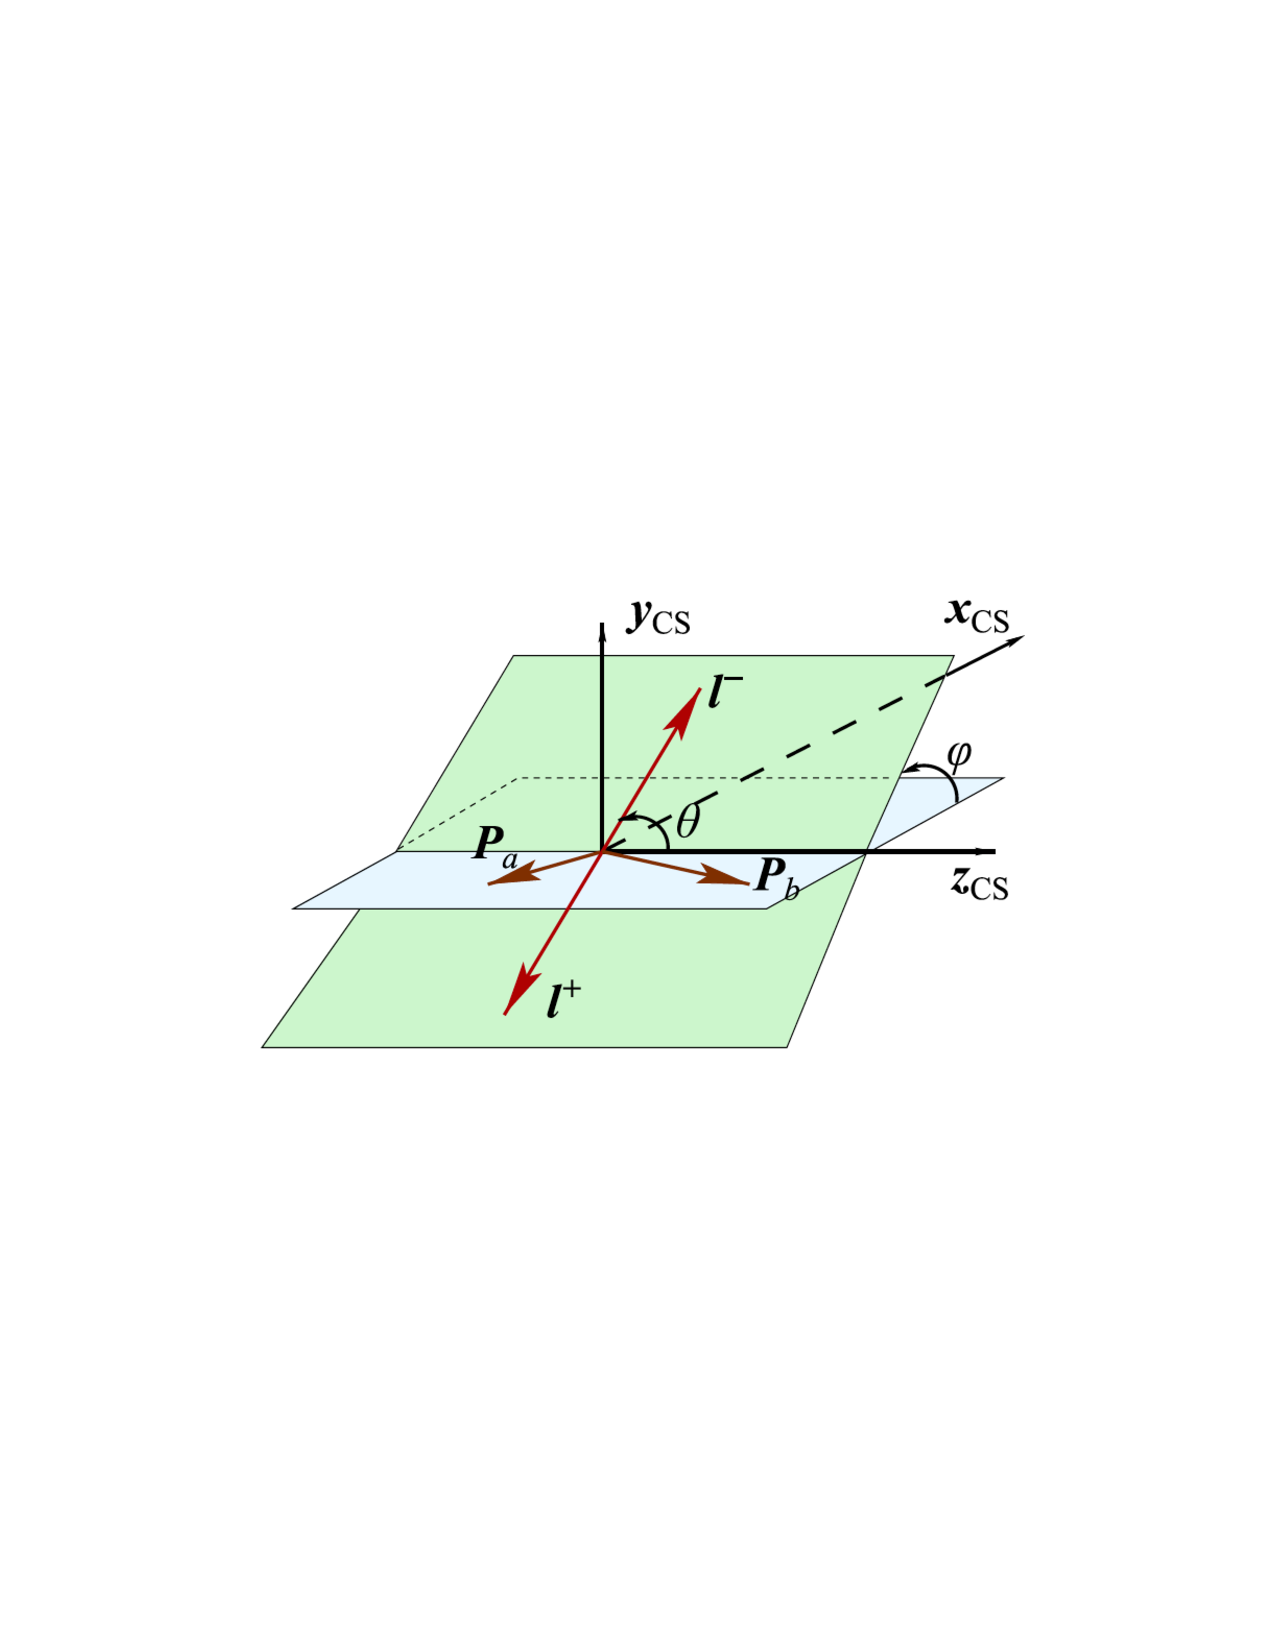
\includegraphics[width=\linewidth, trim=3cm 9cm 3cm 8cm,
      clip]{DY_CSFrame}
    \caption{The Collins-Soper frame is defined in the rest frame of the virtual
      photon where the z-axis bisects the beam and target momentum vectors.}
    \label{fig::DY_CSFrame}%
  \end{subfigure}
\end{figure}

The target frame is defined in the lab frame where the lab frame is rotated so
the beam is along the z-axis and the transverse momentum of the virtual photon
is along the x-axis.  The y-axis in the target frame is then chosen so the
coordinate system is right handed.  The Collins-Soper frame is defined in the
rest frame of the virtual photon where the xz-plane coincides with the hadron
plane and the z-axis is chosen so it bisects the momentum vectors $P_a$ and
$-P_b$.  The CS frame is defined from the target frame as a boost first along
the along z-axis and then a boost along the x-axis so the rest frame of the
virtual photon is reached.  In this way the x-axis of the CS frame is defined
and then the y-axis is again chosen so the coordinate system is right handed.

The leading order model independent Drell-Yan differential cross-section for a
polarized target is~\cite{DYxSection,AKotzininaNote}

\begin{align} \label{equ::DY_ang_dist}
  \frac{d\sigma}{d^4 q \, d \Omega} &=
  \frac{\alpha_{em}^2}{F \, q^2}
  \Big \{ \Big(
   (1 + \cos^2 \theta) \, F_{U}^{1} 
 + (1 - \cos^2 \theta) \, F_{U}^{2} 
 + \sin 2\theta \cos \phi \, F_{U}^{\cos \phi} 
 + \sin^2 \theta \cos 2\phi \, F_{U}^{\cos 2\phi} \Big)
 \nonumber \\
 &+ S_{L} \Big( 
   \sin 2\theta \sin \phi \, F_{L}^{\sin \phi} 
   + \sin^2 \theta \sin 2\phi \, F_{L}^{\sin 2\phi} \Big)
   \nonumber \\
   &+ |S_{T}|
   \Big[ \Big(
     F_{T}^{\sin \phi_S} + \cos^2 \theta \, \tilde{F}_{T}^{\sin \phi_S}
     \Big)\sin \phi_{S} 
     + \Big( F_{T}^{\sin (\phi +\phi_S)} \, \sin(\phi+\phi_S) +
     F_{T}^{(\sin \phi - \phi_S)}\, \sin(\phi-\phi_S) \Big)\sin 2\theta
     \nonumber \\
     & \quad\quad\quad +
     \Big( F_{T}^{\sin (2\phi +\phi_S)}\, \sin(2\phi+\phi_S) +
     F_{T}^{\sin (2\phi - \phi_S)}\, \sin(2\phi-\phi_S) \Big)\sin ^2\theta
     \Big ]
   \Big \},
\end{align}
\noindent
where $F = 4\sqrt{(P_a \cdot P_b)^2 - M_a^2M_b^2}$ is the flux and $\Omega$ is
the solid angle of the outgoing negatively charged muon.  The twelve model
independent structure functions in Eq.~\ref{equ::DY_ang_dist} are labeled as
$F_{Target \; polarization}^{azimuthal \;angle\;coefficient}$.  The phase space
when the TMD regime is valid in DY scattering is when $q_T << q$.  In this
regime the structure functions are equal to a convolution of a beam and a target
TMD function.  The convolution is defined similarly to the SIDIS case,
Eq.~\ref{equ::SIDIS_conv}, as

\begin{align}
  \label{equ::DY_conv}
  \nonumber
      {\cal C}\bigl[ w(k_{aT}, k_{bT}) f_1 \bar{f}_2 \bigr] =
      \frac{1}{N_c} \sum_q e_q^2 \int &d^2 k_{aT} d^2 k_{bT} 
      \delta^{(2)}\bigl(q_T - k_{aT} - k_{bT} \bigr) \\
      &\times w(k_{aT},k_{bT})
        \Big[ f_1^q(x,k_{aT}^2)f_2^{\bar{q}}(x,k_{bT}^2) +
          f_1^{\bar{q}}(x,k_{aT}^2)f_2^{q}(x,k_{bT}^2) \Big],
\end{align}
\noindent
where $N_c = 3$ is the number of color charges and in this notation $f_1$ is a
beam TMD function and $f_2$ is a target TMD function.  The leading order DY
structure functions in the TMD phase space are related to TMD functions
as~\cite{DYxSection}

\begin{align}
  F_{U}^{1} &  =  
  {\cal C}  \big[ f_{1}  \bar{f}_{1} \big]
  &\propto f^{\bar{u}}_{1,Beam} \otimes f^u_{1,Target}, \\
  F_{U}^{\cos 2\phi} &  =  
  {\cal C}  \Bigg[ \frac{2\big( \vec{h} \cdot \vec{k}_{aT} \big) 
                          \big( \vec{h} \cdot \vec{k}_{bT} \big)
                         - \vec{k}_{aT} \cdot \vec{k}_{bT}} {M_{a} M_{b}}  
    h_{1}^{\perp}  \bar{h}_{1}^{\perp} \Bigg]
  &\propto h^{\perp \, \bar{u}}_{1,Beam} \otimes h^{\perp \, u}_{1,Target}, \\
F_{L}^{\sin 2\phi} &  =  
-  {\cal C}  \Bigg[ \frac{2\big( \vec{h} \cdot \vec{k}_{aT} \big) 
                          \big( \vec{h} \cdot \vec{k}_{bT} \big)
                         - \vec{k}_{aT} \cdot \vec{k}_{bT}} {M_{a} M_{b}}  
                  h_{1}^{\perp}  \bar{h}_{1L}^{\perp} \Bigg]
&\propto h^{\perp \, \bar{u}}_{1,Beam} \otimes h^{\perp \, u}_{1L,Target}, \\
F_{T}^{1} &  =   
{\cal C}  \Bigg[ \frac{\vec{h} \cdot \vec{k}_{bT}} {M_{b}}  
  f_{1}  \bar{f}_{1T}^{\perp} \Bigg]
&\propto f^{\bar{u}}_{1,Beam} \otimes f^{\perp \, u}_{1T,Target}, \\
F_{T}^{\sin (2\phi - \phi_S)} &  =  
-  {\cal C}  \Bigg[ \frac{\vec{h} \cdot \vec{k}_{aT}} {M_{a}} 
  h_{1}^{\perp}  \bar{h}_{1} \Bigg]
&\propto h^{\perp \, \bar{u}}_{1,Beam} \otimes h^{u}_{1,Target}, \\
F_{T}^{\sin (2\phi + \phi_S)} &  =  
-  {\cal C}  \Bigg[ \frac{2\big( \vec{h} \cdot \vec{k}_{bT} \big)
                    \big[2 \big( \vec{h} \cdot\vec{k}_{aT} \big)
                         \big( \vec{h} \cdot \vec{k}_{bT} \big)
                        -\vec{k}_{aT} \cdot \vec{k}_{bT} \big]
                   - \vec{k}_{bT}^{2} \big( \vec{h} \cdot \vec{k}_{aT} \big)}
                  {2 M_{a} M_{b}^{2}}  
                  h_{1}^{\perp}  \bar{h}_{1T}^{\perp} \Bigg]
&\propto h^{\perp \, \bar{u}}_{1,Beam} \otimes h^{\perp \, u}_{1T,Target},
\end{align}

\noindent
where $\vec{h} = \vec{q}_T/q_T$ is a unit vector and furthermore the assumption
is made that the beam $\bar{u}$-quark annihilates with the target u-quark.  The
additional leading order structure functions are zero

\begin{equation}
  F_{U}^{2} \quad = \quad F_{U}^{\cos\phi} \quad = \quad F_{L}^{\sin\phi} \quad
  = \quad F_{T}^{2} \quad = \quad F_{T}^{\sin(\phi - \phi_S)} \quad = \quad
  F_{T}^{\sin(\phi + \phi_S)} \quad = 0.
\end{equation}

The differential cross-seciton, Eq.~\ref{equ::DY_ang_dist}, can be rewritten in
terms of asymmetry amplitudes and depolarization factors.  The asymmetry
amplitudes are defined similarly to the case in SIDIS,
Eq.~\ref{equ::asymAmpSIDIS}, and again for the reason that asymmetries can be
determined to a higher precision than structure functions.  For Drell-Yan these
asymmetry amplitudes are

\begin{equation}
  A^{w_i(\phi, \phi_S)}_{Target} = \frac{F^{w_i(\phi,
      \phi_S)}_{Target}}{F_{U}^1+F_{U}^2},
  \label{equ::asymAmpDY}.
\end{equation}
\noindent
The asymmetry amplitudes are the result of different virtual photon
polarizations decaying to final state lepton pair.  The depolarization factor is
defined as the ratio of the virtual photon polarization to produce such an
asymmetry to that of a transversely polarized virtual photon.  The
depolarization is defined for each asymmetry amplitude as

\begin{equation}
  D_{[f(\theta)]} = \frac{f(\theta)}{1+A_U^1\;\cos^2\theta},
\end{equation}
\noindent
where the function $f(\theta)$ corresponds to virtual photon angular decay
responsible for the given asymmetry.  The Drell-Yan differential cross-section,
Eq.~\ref{equ::DY_ang_dist}, now simplifies to~\cite{AKotzininaNote}

\begin{align}
  \frac{d\sigma}{d^4 q \, d \Omega} &=
  \frac{\alpha_{em}^2}{F \, q^2}\hat{\sigma}_U
  \Big \{ \Big(1 + D_{[\sin^2 \theta]} \cos 2\phi \, A_{U}^{\cos 2\phi} \Big)
 \nonumber \\
 &+ S_{L} D_{[\sin^2 \theta]} \sin 2\phi \, A_{L}^{\sin 2\phi}
   \nonumber \\
   &+ |S_{T}|
   \Big[A_{T}^{\sin \phi_S}\;\sin \phi_{S} 
     + \Big( A_{T}^{\sin (2\phi +\phi_S)}\, \sin(2\phi+\phi_S) +
     A_{T}^{\sin (2\phi - \phi_S)}\, \sin(2\phi-\phi_S) \Big)D_{[\sin ^2\theta]}
     \Big ]
   \Big \},
\end{align}
\noindent
where $\hat{\sigma}_U = F^1_U (1+\cos^2\theta)$ is the unpolarized DY
cross-section.


\section{Weighted Asymmetries}
